%%%%%%%%%%%%%%%%%%%% book.tex %%%%%%%%%%%%%%%%%%%%%%%%%%%%%
%
% sample root file for the chapters of your "monograph"
%
% Use this file as a template for your own input.
%
%%%%%%%%%%%%%%%% Springer-Verlag %%%%%%%%%%%%%%%%%%%%%%%%%%


% RECOMMENDED %%%%%%%%%%%%%%%%%%%%%%%%%%%%%%%%%%%%%%%%%%%%%%%%%%%
\documentclass[graybox,envcountchap,sectrefs]{svmono}

% choose options for [] as required from the list
% in the Reference Guide

%\usepackage{mathptmx}
%\usepackage{helvet}
%\usepackage{courier}
%
\usepackage[portuguese]{babel}
\usepackage[utf8]{inputenc}
\usepackage{type1cm}

\usepackage{makeidx}         % allows index generation
\usepackage{graphicx}        % standard LaTeX graphics tool
                             % when including figure files
\usepackage{multicol}        % used for the two-column index
\usepackage[bottom]{footmisc}% places footnotes at page bottom

\usepackage{newtxtext}       % 
\usepackage[varvw]{newtxmath}       % selects Times Roman as basic font
\usepackage{listings}
\usepackage{listingsutf8}
\usepackage{calligra}
\usepackage{multirow}
\usepackage{array}
\usepackage{tabu}
\usepackage{venndiagram}
\usepackage{tikz-cd}
\usepackage{float}
\usepackage{caption}
\usepackage{subcaption}
\usepackage{colortbl}
\usepackage{tikz}
\usepackage{atbegshi}
\usepackage[hidelinks]{hyperref}
\usepackage{setspace}
\usepackage[left=2.5cm,right=2.5cm,top=3cm,bottom=3cm]{geometry}

\newtheorem{teorema}{Teorema}[section]
\newtheorem{lema}{Lema}[section]
\newtheorem{prop}{Proposi\c c\ ̃ao}[section]
\newtheorem{defi}{Defini\c c\ ̃ao}[section]
\newtheorem{obs}{Observa\c c\ ̃ao}[section]
\newtheorem{cor}{Corol\'ario}[section]
\newtheorem{Ex}{Exemplo}[section]

\usetikzlibrary{graphs}
\setlength{\tabcolsep}{5pt}
\definecolor{lightgray}{gray}{0.9}

\DeclareMathOperator{\mat}{Matema}

%s\AtBeginDocument{\AtBeginShipoutNext{\AtBeginShipoutDiscard}}

\begin{document}

\author{Emanuel Mendes Queiroz, Giselle Lopes da Cruz, M\'arcio Ant\^onio de Andrade Bortoloti, Maria Clara Brito dos Reis, Samara Viriato Vilar Dias, Wéllington Moutinho Dias}
\title{Apostila \textit{LaTeX}}
\subtitle{Uma introdu\c c\~ao ao editor de texto \textit{LaTeX}}
\maketitle

\frontmatter%%%%%%%%%%%%%%%%%%%%%%%%%%%%%%%%%%%%%%%%%%%%%%%%%%%%%%

%%%%%%%%%%%%%%%%%%%%%%acknow.tex%%%%%%%%%%%%%%%%%%%%%%%%%%%%%%%%%%%%%%%%%
% sample acknowledgement chapter
%
% Use this file as a template for your own input.
%
%%%%%%%%%%%%%%%%%%%%%%%% Springer %%%%%%%%%%%%%%%%%%%%%%%%%%

\extrachap{Agradecimentos}

Os autores agradecem ao Programa de Educa\c c\~ao Tutorial Institucional da Univesidade Estadual do Sudoeste da Bahia (PETI/UESB) pelas bolsas de estudo e à \textit{Springer Nature} por disponibilizar o template que tornou poss\'ivel a cria\c c\~ao deste material. 

\extrachap{Apresentação}
\noindent O Programa de Educa\c c\~ao Tutorial Institucional de Matem\'atica (PETIMAT) tem como miss\~ao aprimorar os cursos regulares de gradua\c c\~ao na Universidade Estadual do Sudoeste da Bahia (UESB), com o objetivo de proporcionar uma forma\c c\~ao abrangente e de alta qualidade para os alunos envolvidos, mantendo a integra\c c\~ao entre ensino, pesquisa e extens\~ao como um princ\'ipio fundamental do ambiente universit\'ario.

\noindent O PETIMAT se dedica a elevar o padr\~ao da forma\c c\~ao dos estudantes de gradua\c c\~ao e promover o sucesso acad\^emico. Para alcan\c car esses objetivos, o programa oferece, a cada semestre, minicursos voltados principalmente para os alunos matriculados no curso de matem\'atica da UESB. Esses minicursos visam estimular a capacita\c c\~ao de futuros profissionais e docentes, proporcionando-lhes uma qualificação acad\^emica, cient\'ifica, t\'ecnica e tecnol\'ogica. 

\noindent Dentro desse contexto, o PETIMAT desenvolveu o minicurso "Introdução \`a Edi\c c\~ao de Textos usando LaTeX". O objetivo desse minicurso \'e apresentar conceitos e no\c c\~oes iniciais relacionados ao LaTeX, bem como fornecer instru\c c\~oes sobre comandos b\'asicos de formata\c c\~ao de texto e introduzir os principais tipos de documentos cient\'ificos, tais como artigos, monografias, apresenta\c c\~oes (utilizando o beamer) e p\^osteres. A inten\c c\~ao \'e capacitar os participantes para que se tornem aut\^onomos na produ\c c\~ao de seus pr\'oprios textos.

\noindent Este material corresponde \`as notas de aula e serve como um recurso de consulta para os participantes do minicurso. Nesta apostila, est\~ao dispon\'iveis informações detalhadas e comandos necess\'arios para criar e personalizar esses diversos tipos de documentos. Para ter acesso aos diferentes modelos de documentos criados durante o minicurso, basta consultar o nosso reposit\'orio no GitHub:
\begin{center}
    \url{https://github.com/petimatematica/curso_latex}
\end{center}
\noindent Para conhecer mais sobre o trabalho e as publica\c c\~oes do PETIMAT, acesse o nosso site: 
\begin{center}
\url{http://www2.uesb.br/programa/petimatematica/}
\end{center}
e nossa conta oficial no Instagram: 
\begin{center}
\url{https://www.instagram.com/petimatuesb/}
\end{center}
onde est\~ao dispostas informa\c c\~oes detalhadas sobre nossas atividades, projetos, eventos e conte\'udos relacionados ao nosso programa.




\tableofcontents

\mainmatter%%%%%%%%%%%%%%%%%%%%%%%%%%%%%%%%%%%%%%%%%%%%%%%%%%%%%%%



%%%%%%%%%%%%%%%%%%%%% chapter.tex %%%%%%%%%%%%%%%%%%%%%%%%%%%%%%%%%
%
% sample chapter
%
% Use this file as a template for your own input.
%
%%%%%%%%%%%%%%%%%%%%%%%% Springer-Verlag %%%%%%%%%%%%%%%%%%%%%%%%%%
%\motto{Use the template \emph{chapter.tex} to style the various elements of your chapter content.}
\chapter{Introdu\c c\~ao}
\label{intro} % Always give a unique label
% use \chaptermark{}
% to alter or adjust the chapter heading in the running head

\abstract*{Each chapter should be preceded by an abstract (no more than 200 words) that summarizes the content. The abstract will appear \textit{online} at \url{www.SpringerLink.com} and be available with unrestricted access. This allows unregistered users to read the abstract as a teaser for the complete chapter.
Please use the 'starred' version of the new \texttt{abstract} command for typesetting the text of the online abstracts (cf. source file of this chapter template \texttt{abstract}) and include them with the source files of your manuscript. Use the plain \texttt{abstract} command if the abstract is also to appear in the printed version of the book.}

Neste material, exploraremos o sistema TeX, com foco especial no editor de texto \LaTeX. Descobriremos como essa ferramenta pode ser utilizada para criar e formatar uma ampla variedade de documentos, abrangendo desde simples artigos até monografias, apresentações em estilo \emph{beamer} e pôsteres informativos. Ao longo deste guia, iremos explorar as ferramentas essenciais que o \LaTeX{} oferece, permitindo produzir documentos profissionais.

\section{O que \'e o LaTeX?}
\label{sec:1}

O \TeX\ é uma not\'avel linguagem de marcação, concebida e apresentada por Donald Knuth em 1978. Essa linguagem trouxe consigo um novo padrão de qualidade tipográfica, porém, logo após seu lançamento, surgiu uma demanda por uma abordagem mais simplificada e acessível. Isso se deve ao fato de que, apesar das melhorias na tipografia, o \TeX\ apresentava uma curva de aprendizado acentuada e necessitava de conhecimento em programação, o que restringia sua adoção a um público mais especializado.

\noindent Esse cenário deu origem ao \LaTeX, uma evolução do \TeX\ desenvolvida por Leslie Lamport na década de 1980. O \LaTeX\ foi projetado para facilitar a produção de documentos de alta qualidade, em que os autores poderiam focar no conteúdo em vez de se preocupar com os detalhes de formatação. Com comandos mais intuitivos e uma estrutura de documento modular, o \LaTeX\ rapidamente se tornou uma ferramenta fundamental para a comunidade acadêmica e científica, onde a apresentação precisa de fórmulas matemáticas e citações bibliográficas era essencial.

\noindent O desenvolvimento posterior do \LaTeX\ representou uma resposta à necessidade de tornar a composição de documentos tipográficos mais acessível e eficaz, desempenhando um papel significativo na evolução da produção textual, especialmente na esfera acadêmica e científica.


\section{Vantagens de usar o LaTeX}
\noindent O \LaTeX \ oferece diversas vantagens que o tornam uma escolha assertiva para a cria\c c\~ao de documentos. Neste contexto, uma de suas principais vantagens \'e a versatilidade, adequada para a cria\c c\~ao de diversos tipos de documentos. Al\'em disso, o \LaTeX \ \'e amplamente reconhecido por sua capacidade de lidar com as nota\c c\~oes matem\'aticas de maneira pr\'atica e eficiente, em que \'e poss\'ivel escrever equa\c c\~oes complexas e s\'imbolos matem\'aticos com facilidade. Ademais, ao contr\'ario de muitos editores de texto que possuem m\'ultiplas barras de ferramentas, o \LaTeX \ oferece uma abordagem mais simplificada, em que \'e possível editar todo o texto em uma \'unica aba.
\section{Instalação}
\label{sec:2}

\noindent A instala\c c\~ao do \LaTeX\ \'e dividida em duas partes, pois envolve a configura\c c\~ao de dois componentes essenciais: o compilador e o editor. 

\noindent Ao escrever um texto em \LaTeX\, estamos essencialmente criando um c\'odigo-fonte que descreve a estrutura e o conte\'udo do documento. Esse c\'odigo-fonte cont\'em comandos que instruem o \LaTeX\ sobre como formatar o texto. Para isso, \'e necess\'ario compilar o texto, ou seja, o \LaTeX\ l\^e o c\'odigo-fonte, interpreta os comandos e gera um arquivo de sa\'ida.

\noindent O editor \'e o respons\'avel por oferecer uma s\'erie de recursos que simplificam a cria\c c\~ao e a formata\c c\~ao de documentos, como preenchimento autom\'atico de comandos, ajuda na identifica\c c\~ao de erros no c\'odigo e atalhos para a compila\c c\~ao instant\^anea. Al\'em disso, os editores frequentemente organizam a visualiza\c c\~ao do documento, permitindo a vis\~ao da \'area de edi\c c\~ao e do documento final lado a lado, facilitando a identifica\c c\~ao de poss\'iveis ajustes.

\subsection{Instala\c c\~ao do MiKTeX no Windows}

\noindent O MiKTeX \'e o respons\'avel por compilar as entradas em \TeX\ no Windows e gerar o documento j\'a formatado. Para ainstalação, acesse o site oficial do MiKTeX 
\begin{center}
\url{https://miktex.org/download}
\end{center}

\noindent e escolha o sistema operacional correspondente ao seu dispositivo. Com isso, basta clicar em "Download" \ e, em seguida, executar o arquivo de instal\c c\~ao j\'a baixado.
\noindent Ap\'os isso clique em "Avan\c car" \ no termo com as condições para o uso e  selecione "Complete MiKTeX” para baixar a versão completa. o MixTeX será baixado para o local selecionado anteriormente.
\subsection{Intala\c c\~ao do MiKTeX no Linux}
\noindent \'E importante observar que o MikTeX n\~ao possui uma vers\~ao nativa para sistemas LinuX. Em virtude disso, recomendamos o tutorial disposto no site oficial do MiKTeX
\begin{center}
\url{https://miktex.org/download}
\end{center}
em que ser\'a poss\'ivel encontrar informa\c c\~oes espec\'ificas para usu\'arios do LinuX, incluindo instru\c c\~oes passo a passo sobre como configurar e ultilizar o MiKTeX neste sistema.
\subsection{Instala\c c\~ao do MacTeX no Macbook}
\noindent Acesse o site oficial do MacTeX:
\begin{center}
\url{https://tug.org/mactex/mactex-download.html}.   
\end{center}
Baixe o arquivo de instala\c c\~ao \textit{MacTeX.pkg} e em seguida, execute-o. Ap\'os isso, o assistente de instalação do MacTeX será aberto. Siga as instruções na tela para concluir a instalação. Elas incluirão a aceitação do contrato de licença e a escolha do diretório de instalação. Vale ressaltar que o usu\'ario deve verificar a vers\~ao do seu Macbook para baixar a vers\~ao do MacTeX correspondente.

\section{Editores LaTeX}
\label{sec:3}
\subsection{TeXWorks}
\noindent Acesse o site oficial do TeXWorks 
\begin{center}
\url{https://www.tug.org/texworks/}    
\end{center}
\noindent  e baixe a vers\~ao apropriada para o seu sistema operacional (Windows, Mac ou Linux). Apo\'os isso, execute o arquivo e siga as instru\c c\~oes para concluir a instala\c c\~ao padr\~ao.

\subsection{TexStudio}
Acesse o site oficial do TeXStudio
\begin{center}
\url{https://www.texstudio.org/}   
\end{center}
e baixe a vers\~ao apropriada para o seu sistema operacional (Windows, Mac ou Linux). Ap\'os isso, execute o arquivo e siga as instru\c c\~oes para concluir a instala\c c\~ao padr\~ao.
\subsection{Overleaf}
O Overleaf é uma plataforma online para escrita em LaTeX que não requer instala\c c\~ao local. Basta criar uma conta no site do Overleaf 
\begin{center}
    \url{https://www.overleaf.com/project}
\end{center}
e começar a escrever imediatamente, pois ele entende a linguagem \LaTeX e formata o texto automaticamente, sendo possível exportá-lo para um arquivo em PDF ou outros formatos para imprimir ou compartilhar.
\section{T\'opicos b\'asicos do LaTeX}
\label{sec:4}
O \LaTeX\ oferece uma maneira estruturada de criar documentos. Atrav\'es dos comandos e ambientes, podemos definir a formata\c c\~ao, a organiza\c c\~ao e os elementos do nosso documento de forma precisa e eficaz.

\subsection{Pre\^ambulo}
\label{sec:5}
No \LaTeX, o pre\^ambulo representa as configura\c c\~oes iniciais do c\'odigo onde s\~ao definidas diretrizes globais, formata\c c\~ao e informa\c c\~oes cruciais que permeiam todo o documento a ser criado. Ele \'e o respons\'avel por dar forma, estilo e personalidade \`a cria\c c\~ao textual. Nele, não deve ser escrito o conte\'udo principal do texto, mas devem ser declaradas as regras que v\~ao orientar a apresenta\c c\~ao, como a escolha do tipo de documento ou os pacotes a serem utilizados, que abordaremos posteriormente. No pre\^ambulo, deve ser definido o tipo de documento que está sendo criado, como um artigo, um relatório ou um livro.  Isso pode ser feito com o comando \texttt{\textbackslash documentclass\{\}}.

\subsection{Elementos iniciais do texto}
No \LaTeX, um documento \'e organizado por meio de comandos espec\'ificos. Para inciar o texto, deve ser utilizado o comando \texttt{\textbackslash begin\{document\}} e para finalizar, o comando \texttt{\textbackslash end\{document\}}. Tudo entre esses comandos será processado e exibido no documento.

\noindent A barra invertida (\texttt{\textbackslash}) \'e usada para indicar comandos no \LaTeX. No preâmbulo, o comando \texttt{\textbackslash title\{\}} \'e utilizado para definir o t\'itulo do documento, j\'a o comando \texttt{\textbackslash author\{\}} define o nome do autor e \texttt{\textbackslash date\{\}} define a data. Essas informações serão usadas posteriormente para criar o cabe\c calho do texto.

\noindent Outro fator importante \'e o s\'imbolo \verb|%|, usado para indicar coment\'arios ao longo da escrita. Quando usado, qualquer texto seguido de \verb|%| em uma linha n\~ao ser\'a processado pelo compilador, e portanto, n\~ao aparecer\'a no documento final.


\section{Pacotes e Extens\~oes}
\label{sec:6}
 Os Pacotes e extensões no \LaTeX\ são conjuntos de comandos e funcionalidades pr\'e-definidos que permitem a inclus\~ao de recursos adicionais ao seu documento. Eles abrangem desde a manipula\c c\~ao de imagens, tabelas, equa\c c\~oes matem\'aticas complexas at\'e a inser\c c\~ao de c\'odigos-fonte e algoritmos. Essas extens\~oes s\~ao criadas por membros da comunidade \LaTeX\ para facilitar tarefas espec\'ificas e adicionar recursos especializados. Atrav\'es da incorpora\c c\~ao de pacotes e extens\~oes, pode-se adicionar funcionalidades avan\c cadas, formatar elementos espec\'ificos e aprimorar significativamente a qualidade e a est\'etica do trabalho. 

\section{Ambientes}
\label{sec:7}
\noindent Um ambiente \'e uma estrutura delimitada que define a maneira que o conte\'udo deve ser formatado e exibido. O \LaTeX\ oferece uma variedade de ambientes que permite formatar diferentes partes do documento de maneira espec\'ifica. Esses ambientes fornecem estruturas de textos, listas, equa\c c\~oes e outros elementos. O s\'imbolo \verb|$|, por exemplo, desempenha um papel fundamental na marca\c c\~ao do \textit{ambiente matemático}. Quando envolvemos uma express\~ao ou equa\c c\~ao entre \verb|$$|, o \LaTeX\ reconhece que o conte\'udo deve ser interpretado como c\'odigo matem\'atico. Ao longo deste material, ser\~ao abordados outros ambientes. Abaixo, seguem exemplos de ambientes que n\~ao necessitam de outros comandos e pacotes no pre\^ambulo. 
% \begin{trailer}{Teorema}
% Ambiente utilizado para enunciar teoremas.
% \begin{verbatim}\begin{theorem}
% ...
% \end{theorem}\end{verbatim}

% \end{trailer}
% \begin{trailer}{Lema}
% Ambiente utilizado para enunciar Lemas.
% \begin{verbatim}\begin{lemma}
% ...
% \end{lemma}\end{verbatim}
% \end{trailer}
% \begin{trailer}{Defini\c c\~oes}
% Ambiente utilizado para enunciar defini\c c\~oes.
% \begin{verbatim}\begin{definition}
% ...
% \end{definition}\end{verbatim}

% \end{trailer}
% \begin{trailer}{Equa\c c\~oes}
% Ambiente utilizado para criar equa\c c\~oes.
% \begin{verbatim}\begin{equation}
% ...
% \end{equation}\end{verbatim}
% Ambiente utilizado para alinhar equa\c c\~oes verticalmente.
% \begin{verbatim}\begin{aling}
% ...
% \end{aling}\end{verbatim}

% \end{trailer}
\begin{trailer}{Listas n\~ao numeradas}
\begin{verbatim}
\begin{itemize}
...
\end{itemize}
\end{verbatim}
\end{trailer}

\begin{trailer}{Listas numeradas}
\begin{verbatim}
\begin{enumerate}
    \item{}
...
\end{enumerate}
\end{verbatim}
\end{trailer}

\noindent Neste exemplos, o comando utilizado para adicionar os itens da lista \'e definido por \texttt{\textbackslash item\{\}}.
% \begin{trailer}{Cita\c c\~oes}
% Ambiente utilizado para citar textos longos, onde a cita\c c\~ao \'e recuada em rela\c c\~ao ao restante do texto.
% \begin{verbatim}\begin{quote}
% ...
% \end{quote}\end{verbatim}

% \end{trailer}

%%%%%%%%%%%%%%%%%%%%% chapter.tex %%%%%%%%%%%%%%%%%%%%%%%%%%%%%%%%%
%
% sample chapter
%
% Use this file as a template for your own input.
%
%%%%%%%%%%%%%%%%%%%%%%%% Springer-Verlag %%%%%%%%%%%%%%%%%%%%%%%%%%
%\motto{Use the template \emph{chapter.tex} to style the various elements of your chapter content.}
\chapter{Formatação de texto}
\label{intro} % Always give a unique label
% use \chaptermark{}
% to alter or adjust the chapter heading in the running head

Em todo texto é necessário elementos para format\'a-lo de acordo com as necessidades de cada escritor. Assim,
neste capítulo, apresentaremos os tópicos básicos para formatação de qualquer texto em \LaTeX{}.

\section{Tamanho e estilo de fonte}
\label{sec:1}
Um dos aspectos mais importantes quando se está formatando um texto é o tamanho da fonte. Abaixo, iremos mostrar as principais formas de fazer essas alterações em um texto utilizando o \LaTeX{}.\\

\begin{center}
	\begin{tabular}{lcc}
		\hline
	\textbf{Comando}	&  \textbf{Resultado}\\
		\hline
	\verb|\tiny{Exemplo}| &  \tiny Exemplo\\ 
		\hline
	\verb|\scriptsize{Exemplo}|	& \scriptsize Exemplo \\
		\hline
	\verb|\footnotesize{Exemplo}|	&  \footnotesize Exemplo\\
		\hline
	\verb|\small{Exemplo}|	& \small Exemplo \\
		\hline
	\verb|\normalsize{Exemplo}|	& \normalsize Exemplo \\
		\hline
	\verb|\large{Exemplo}|	& \large Exemplo \\
		\hline
	\verb|\Large{Exemplo}|	& \Large Exemplo \\
		\hline
	\verb|\LARGE{Exemplo}|	& \LARGE Exemplo \\
		\hline
	\verb|\huge{Exemplo}|	& \huge Exemplo \\
		\hline
	\verb|\Huge{Exemplo}|	& \Huge Exemplo \\
		\hline
	\end{tabular}
\end{center}

\noindent Para deixar o texto em negrito é necessário usar o comando \verb|\textbf|. Veja o exemplo:
\begin{trailer}{Texto em negrito}

\begin{verbatim}\begin{document}
    \textbf{Exemplo}
\end{documument}\end{verbatim}
\end{trailer}

\noindent Para deixar o texto em itálico é necessário usar o comando \verb|\textit|. Veja o exemplo:
\begin{trailer}{Texto em itálico}
\begin{verbatim}\begin{document}
    \textit{Exemplo}
\end{document}\end{verbatim}
\end{trailer}

\noindent Para deixar o texto sublinhado é necessário usar o comando \verb|\underline|. Veja o exemplo:
\begin{trailer}{Texto sublinhado}
\begin{verbatim}\begin{document}
    \underline{Exemplo}
\end{document}\end{verbatim}
\end{trailer}

\noindent Para deixar o texto com alguma cor diferente é necessário que no preâmbulo esteja o pacote \verb|xcolor| e em seguida no texto com o comando \verb|\textcolor{}{}|, sendo o primeiro argumento a cor que deseja e no segundo o texto que deseja colorir. Veja o exemplo a seguir:
\begin{trailer}{Cor no texto}
\begin{verbatim}
\usepackage{xcolor}  
\begin{document}
    \textcolor{red}{Texto}
\end{document}
\end{verbatim}
\end{trailer}

%COMO FICARIA 
%
\section{Espaçamento entre linhas}
Para alterar o espaçamento entre linhas é preciso adicionar no preâmbulo do texto o pacote \verb|setspace| e no  corpo do texto adicionar um dos seguintes comandos:
\begin{itemize}
    \item \verb|\singlespacing| - Espaçamento simples
    \item \verb|\onehalfspacing| - Espaçamento de $1,5$
    \item \verb|\doublespacing| - Espaçamento duplo
\end{itemize}

\begin{trailer}{Espaçamento entre linhas}
\begin{verbatim}
\usepackage{setspace}  
\begin{document}
    \singlespacing
    Copiar texto desejado. \\
    O texto terá espaçamento simples 

    %Para alterar espaçamento basta adicionar o outro

    \onehalfspacing
    Copiar texto desejado.\\
    O texto terá espaçamento de 1,5
\end{document}
\end{verbatim}
\end{trailer}

\noindent Se você deseja alterar o espaçamento apenas para um trecho específico de texto (e não para todo o documento), você pode usar os ambientes \verb|singlespace|, \verb|onehalfspace| e \verb|doublespace|. 

\section{Hifenização}
Em um texto em \LaTeX{} a separação silábica é feita de forma automática, visto que a linguagem já é automatizada para que possa ser feito em qualquer idioma. Basta utilizar no preâmbulo o pacote \verb|\usepackage[portuguese]{babel}|. No entanto, caso se queira fazer a hifenização de forma manual de uma palavra é preciso utilizar o comando \verb|\hyphenation{e-xem-plo}| no preâmbulo. 


\section{Ajuste de margens}
Em um texto em \LaTeX{} é preciso ajustar as margens de acordo com as necessidades de cada escritor. Assim, para configurar as margens é necessário inserir no preâmbulo  o pacote \verb|\usepackage{geometry}|. Veja o exemplo abaixo:
\begin{trailer}{Ajustando margens}
\begin{verbatim}
\usepackage[left=2cm,right=2cm,top=3cm,bottom=3cm]{geometry}
%Defina a configuração das margens

\begin{document}
   Inserir texto.
\end{document}
\end{verbatim}
\end{trailer}

\section{Alinhamento do texto}
O alinhamento em um texto é importante, pois distrubui o texto uniformemente entre as margens. Para se ter um alinhamento à esquerda, à direita ou centralizado em um trecho do texto é preciso inserir o texto dentro dos ambientes citados abaixo.
\begin{trailer}{Alinhamento}
\begin{verbatim}
\begin{document}
    \begin{flushleft}
    Trecho alinhado à esquerda
    \end{flushleft}

    \begin{flushright}
    Trecho alinhado à direita
    \end{flushright}

    \begin{center}
    Trecho centralizado
    \end{center}
\end{document}
\end{verbatim}
\end{trailer}

\noindent Para se fazer o alinhamento do texto todo é necessário inserir os seguintes comandos antes do texto:

\begin{trailer}{Alinhamento em todo texto}
\begin{verbatim}
\begin{document}
\raggedleft   %alinhamento à esquerda
\raggedright  %alinhamento à direita
\centering    %centralizado
%Selecione algum desses alinhamentos e inicie a escrita.

Escrever texto
\end{document}
\end{verbatim}
\end{trailer}

\noindent Para que o texto seja escrito de forma justificada, é necessário inserir no preâmbulo o pacote \verb|ragged2e| e utilizar o comando \verb|\justifying| antes de iniciar 
a escrita. Veja o exemplo abaixo:

\begin{trailer}{Alinhamento}
\begin{verbatim}
\usepachege{ragged2e}
\begin{document} \justifying 

Escrever texto que será justificado.

\end{document}
\end{verbatim}
\end{trailer}

\section{Inserir cabeçalho, rodapé e número de páginas}
Em diversos textos, é necessário que tenha cabeçalho, rodapé e indica\c c\~ao do número de páginas para uma melhor organização do texto. Na escrita \LaTeX{} essas configurações são feitas de forma simples e rápida.

\subsection{Cabeçalho e rodapé}
Para inserir cabeçalho e rodapé no texto em \LaTeX{} é necessário inserir no preâmbulo o pacote \verb|fancyhdr| e, em seguida, ainda no preâmbulo, colocar\verb|\pagestyle{fancy}| para que o estilo da página siga a fórmula dada pelo pacote \verb|fancyhdr|. Veja o exemplo

\begin{trailer}{Cabeçalho e rodapé}
\begin{verbatim}
\pagestyle{fancy} % Define o estilo de página como "fancy"
\fancyhf{} % Limpa todos os estilos de cabeçalho e rodapé atuais

% Configuração do cabeçalho
\fancyhead[L]{Cabeçalho à esquerda}
\fancyhead[C]{Cabeçalho no centro}
\fancyhead[R]{Cabeçalho à direita}

% Configuração do rodapé
\fancyfoot[L]{Rodapé à esquerda}
\fancyfoot[C]{Rodapé no centro}
\fancyfoot[R]{Rodapé à direita}

% Linha superior do cabeçalho
\renewcommand{\headrulewidth}{0.4pt}

% Linha inferior do rodapé
\renewcommand{\footrulewidth}{0.4pt}
\end{verbatim}
\end{trailer}

\noindent Para fazer as configurações para o estilo, podemos usar os comandos \verb|lhead|, \verb|rhead|, \verb|lfoot|, \verb|cfoot| e \verb|rfoot| para que seja possível definir o conteúdo que vai ser inserido no cabeçalho e no rodapé em páginas distintas do texto. Já para inserir em uma página específica, basta usar o comando \verb|pagestyle{fancy}|. Veja o exemplo de como colocar cabeçalho e rodapé:

\begin{trailer}{Exemplo}
\begin{verbatim}
\usepackage{fancyhdr}
\pagestyle{fancy}
\fancyhf{}
\fancyhead[L]{Cabeçalho à esquerda}
\fancyhead[C]{Cabeçalho no centro}
\fancyhead[R]{Cabeçalho à direita}
\fancyfoot[L]{Rodapé à esquerda}
\fancyfoot[C]{Rodapé no centro}
\fancyfoot[R]{Rodapé à direita}
\renewcommand{\headrulewidth}{0.4pt}
\renewcommand{\footrulewidth}{0.4pt}
\begin{document}

 Seu conteúdo vai aqui.

\end{document}
\end{verbatim}
\end{trailer}

\subsection{Número de página}
Para inserir número nas páginas no texto em \LaTeX{}, é preciso inserir no preâmbulo o pacote \verb|fancyhdr|, já visto anteriormente. Em seguida, para exibir os números nas páginas, basta inserir o comando \verb|\thepage|. Veja exemplo:
\begin{trailer}{Número nas páginas}
\begin{verbatim}
\usepackage{fancyhdr}

\pagestyle{fancy}
\fancyhf{}
\fancyhead[L]{Cabeçalho à esquerda}
\fancyhead[C]{Cabeçalho no centro}
\fancyhead[R]{Cabeçalho à direita}
\fancyfoot[L]{Rodapé à esquerda}
\fancyfoot[C]{\thepage} % Insere o número da 
página no centro do rodapé
\fancyfoot[R]{Rodapé à direita}
\renewcommand{\headrulewidth}{0.4pt}
\renewcommand{\footrulewidth}{0.4pt}

\begin{document}

Seu conteúdo vai aqui.

\end{document}

\end{verbatim}
\end{trailer}

\noindent Neste exemplo, o comando \verb|\fancyfoot[C]{\thepage}| insere o número da página no centro do rodapé.

\section{Exercícios}

1. Escreva o texto abaixo.\\

\noindent Lorem ipsum dolor sit amet, \textbf{\textit{\underline{consectetur adipiscing elit}}}. Phasellus vitae bibendum libero. Sed vestibulum metus vitae massa fringilla, vel interdum nisi dictum. \textcolor{blue}{\textit{Maecenas vel neque sed orci venenatis tristique. Fusce ut condimentum libero, in tincidunt libero.}} Sed varius, arcu in fermentum hendrerit, sapien urna fringilla nulla, id consequat sapien odio eu justo. Vivamus auctor suscipit lectus.\\
\doublespacing

\noindent 2. Deixe o texto acima centralizado.\\
3. Coloque espaçamento entre as linhas de 1,5.



%%%%%%%%%%%%%%%%%%%%% chapter.tex %%%%%%%%%%%%%%%%%%%%%%%%%%%%%%%%%
%
% sample chapter
%
% Use this file as a template for your own input.
%
%%%%%%%%%%%%%%%%%%%%%%%% Springer-Verlag %%%%%%%%%%%%%%%%%%%%%%%%%%
%\motto{Use the template \emph{chapter.tex} to style the various elements of your chapter content.}
\chapter{T\'opicos Espec\'ificos}
\label{intro} % Always give a unique label
% use \chaptermark{}
% to alter or adjust the chapter heading in the running head

Tendo em vista o que foi visto no capítulo anterior, é possível perceber que em um texto em \LaTeX{} a formatação é algo muito importante para que o texto final fique da forma desejada. Neste capítulo, será discutido sobre alguns tópicos específicos necessários para a escrita.

\section{Acentua\c c\~ao}
\label{sec:2}
Em \LaTeX, existem duas maneiras de se acentuar as palavras. A primeira forma é manualmente e a segunda é da forma tradicional. Para escrever de forma manual, existe um modelo universal em \LaTeX. Veja o exemplo abaixo:
\begin{trailer}{Acentuação manual}
\begin{verbatim}
\begin{document}
%Colocar  ~, ç
Acentua\c c\~ao  

%Colocar ´, `, ^
S\'ilaba  %aspas simples
\`a       %o acento grave
Jud\^o    %o acento circunflexo

\end{document}\end{verbatim}
\end{trailer}
 \noindent Já para colocar a acentuação de forma direta pelo teclado basta acrescentar no preâmbulo o pacote \verb|\usepackage[utf8]{inputenc}|. 

\section{Se\c c\~oes e subse\c c\~oes}
Dentro do ambiente \verb|document|, podemos usar comandos como \verb|section{}| para criar se\c c\~oes no documento e \verb|subsection{}| para criar subse\c c\~oes. As se\c c\~oes ajudam a organizar o conte\'udo em partes distintas, facilitando a leitura e compreens\~ao. Veja o exemplo:

\begin{trailer}{Seção e subseção}
\begin{verbatim}\begin{document}
    \section{Nome da seção}
    Texto
    
    \subsection{Nome da subseção}
    Texto
\end{document}\end{verbatim}
\end{trailer}
\section{Ambientes de equa\c c\~ao}
Em textos matemáticos é inevitavél a escrita de equações. E uma das vantagens da escrita em \LaTeX{} é o fato das equações ficarem organizadas. No \LaTeX{} podemos utilizar os seguintes ambientes para a escrita matemática: \verb|equation|, \verb|eqnarray|, \verb|array|, \verb|align|, \verb|gather| ou utilizar \verb|$equação$|. Veja um exemplo abaixo:

\begin{trailer}{Ambiente de equação}
No ambiente \verb|equation| não é necessário usar \verb|$$|, pois já é um ambiente matemático.
\begin{verbatim}\begin{document}
% Equação numerada
    \begin{equation} 
    x+y=56
    \end{equation}   
    
% Equação não numerada
    \begin{equation*} 
    x+y=56
    \end{equation*}
\end{document}\end{verbatim}
\end{trailer}

\begin{trailer}{Resultado}
\noindent Equação numerada
    \begin{equation} 
    x+y=56
    \end{equation}   
    
\noindent Equação não numerada
    \begin{equation*} 
    x+y=56
    \end{equation*} 
\end{trailer}

\subsection{Alinhamento de equa\c c\~oes}
\noindent Ao escrever as equações em um texto, às vezes é necessário alinhá-las. No \LaTeX{}, para se alinhar as equações, é preciso utilizar o pacote \verb|\usepackage{amsmath}| e o ambiente \verb|align|.\\
No ambiente \verb|align| não precisa usar \verb|$$|, pois já é um ambiente matemático. Assim, quando temos duas ou mais equações, podemos alinhá-las da seguinte forma: 

\begin{trailer}{Alinhar equação}
\begin{verbatim}\begin{document}
    \begin{align*} 
    2x + 3y &= 7 
    3x - 2y &= 4
    \end{align*}

\end{document}
\end{verbatim}
\end{trailer}

\noindent Obteremos o seguinte resultado: 
\begin{align*}
    2x + 3y &= 7 \\
    3x - 2y &= 4
\end{align*}
% \begin{trailer}{Outro exemplo}
% \noindent 
%     \begin{gather}
%           x+y=56 
%     \end{gather} 
 
% \end{trailer}

\noindent Para especificar onde será o alinhamento na próxima linha se utiliza \verb|&| antes da parte que deseja alinhar

\section{Defini\c c\~ao de novos comandos}
Na escrita matemática podem aparecer Teoremas, Lemas, Corolários, Proposições, entre outros. No \LaTeX{}, é possível definir esses ambientes no preâmbulo e inseri-los ao longo do texto de acordo com a necessidade. Veja o exemplo abaixo:

\begin{trailer}{Novos comandos}

\begin{verbatim}
\newtheorem{definition}{Defini\c c\~ao}[section]
\newtheorem{theorem}{Teorema}[section]
\newtheorem{cor}{Corol\'ario}[section]
\newtheorem{lemma}{Lema}[section]
\newtheorem{prop}{Proposi\c c\~ao}[section]
\newtheorem{Ex}{Exemplo}[section]
\newtheorem{Remark}{Observa\c c\~ao}[section]

\begin{document}
    \begin{theorem}
    Enunciado do teorema 
    \end{theorem}
    
% Para os outros comandos se faz da mesma forma

\end{document}\end{verbatim}
\end{trailer}

\begin{trailer}{Resultado}
   \begin{teorema}
  Enunciado do teorema
   \end{teorema}
\end{trailer}

\eject
\enlargethispage{24pt}




%%%%%%%%%%%%%%%%%%%%% chapter.tex %%%%%%%%%%%%%%%%%%%%%%%%%%%%%%%%%
%
% sample chapter
%
% Use this file as a template for your own input.
%
%%%%%%%%%%%%%%%%%%%%%%%% Springer-Verlag %%%%%%%%%%%%%%%%%%%%%%%%%%
%\motto{Use the template \emph{chapter.tex} to style the various elements of your chapter content.}
\chapter{Matem\'atica e S\'imbolos}
\label{intro} % Always give a unique label
% use \chaptermark{}
% to alter or adjust the chapter heading in the running head

Neste cap\'{i}tulo, apresentaremos os s\'{i}mbolos e operadores utilizados nas seções seguintes. Equações b\'{a}sicas serão constru\'{i}das e, por fim, exerc\'{i}cios serão propostos ao leitor para que o mesmo possa verificar o seu progresso.

\section{S\'{i}mbolos}
\label{sec:1}
Apesar do nome do cap\'{i}tulo ser chamado de "Matem\'{a}tica e S\'{i}mbolos", os s\'{i}mbolos ser\~{a}o apresentados primeiro por raz\~{o}es did\'{a}ticas. Apesar disso, n\~{a}o se espera e nem se recomenda que o leitor memorize todos os comandos. Use esta seç\~{a}o apenas como um material para consulta, pois acreditamos que a memorizaç\~{a}o deve ocorrer em virtude da experi\^{e}ncia de uso do \LaTeX.

\noindent A lista a seguir n\~{a}o \'{e} completa, por isso, acesse o site \verb|https://app.mettzer.com/| \verb|latex|, os ap\^{e}ndices A, B e C de \cite{gratzer2007more}, ou ainda, \cite{downes2002short} para mais informaç\~{o}es. Para ter acesso a todos os s\'imbolos a seguir é necess\'ario usar os pacotes \verb|amsmath|, \verb|amsthm|, \verb|amsfonts| e \verb|amssymb|. 

\subsection{Fonte Mathbb}
\begin{equation*}
    \mathbb{A}\mathbb{B}\mathbb{C}\mathbb{D}\mathbb{E}\mathbb{F}\mathbb{G}\mathbb{H}\mathbb{I}\mathbb{J}\mathbb{K}\mathbb{L}\mathbb{M}\mathbb{N}\mathbb{O}\mathbb{P}\mathbb{Q}\mathbb{R}\mathbb{S}\mathbb{T}\mathbb{U}\mathbb{V}\mathbb{W}\mathbb{X}\mathbb{Y}\mathbb{Z}
\end{equation*}

\subsubsection{Fonte Mathbf}
\begin{equation*}
    \mathbf{A}\mathbf{B}\mathbf{C}\mathbf{D}\mathbf{E}\mathbf{F}\mathbf{G}\mathbf{H}\mathbf{I}\mathbf{J}\mathbf{K}\mathbf{L}\mathbf{M}\mathbf{N}\mathbf{O}\mathbf{P}\mathbf{Q}\mathbf{R}\mathbf{S}\mathbf{T}\mathbf{U}\mathbf{V}\mathbf{W}\mathbf{X}\mathbf{Y}\mathbf{Z}
\end{equation*}
\begin{equation*}
    \mathbf{a}\mathbf{b}\mathbf{c}\mathbf{d}\mathbf{e}\mathbf{f}\mathbf{g}\mathbf{h}\mathbf{i}\mathbf{j}\mathbf{k}\mathbf{l}\mathbf{m}\mathbf{n}\mathbf{o}\mathbf{p}\mathbf{q}\mathbf{r}\mathbf{s}\mathbf{t}\mathbf{u}\mathbf{v}\mathbf{w}\mathbf{x}\mathbf{y}\mathbf{z}
\end{equation*}

\subsection{Letras hebraicas}
\begin{equation*}
    \aleph \; \verb|\aleph| \quad \beth \; \verb|\beth| \quad \daleth \; \verb|\daleth| \quad \gimel \; \verb|\gimel|
\end{equation*}

\newpage
\subsection{Letras gregas}

\begin{equation*}
    \begin{matrix}
        \alpha \; \verb|\alpha     | & \Theta \; \verb|\Theta    | & \varXi \; \verb|\varXi   | & \Upsilon \; \verb|\Upsilon   |\\
        \beta \; \verb|\beta      | & \vartheta \; \verb|\vartheta | & \pi \; \verb|\pi      | & \varUpsilon \; \verb|\varUpsilon|\\
        \Gamma \; \verb|\Gamma     | & \varTheta \; \verb|\varTheta | & \Pi \; \verb|\Pi      | & \phi \; \verb|\phi       |\\
        \varGamma \; \verb|\varGamma  | & \iota \; \verb|\iota     | & \varpi \; \verb|\varpi   | & \Phi \; \verb|\Phi       |\\
        \digamma \; \verb|\digamma   | & \kappa \; \verb|\kappa    | & \varPi \; \verb|\varPi   | & \varphi \; \verb|\varphi    |\\
        \delta \; \verb|\delta     | & \varkappa \; \verb|\varkappa | & \rho \; \verb|\rho     | & \varPhi \; \verb|\varPhi    |\\
        \Delta \; \verb|\Delta     | & \lambda \; \verb|\lambda   | & \varrho \; \verb|\varrho  | & \chi \; \verb|\chi       |\\
        \varDelta \; \verb|\varDelta  | & \Lambda \; \verb|\Lambda   | & \sigma \; \verb|\sigma   | & \psi \; \verb|\psi       |\\
        \epsilon \; \verb|\epsilon   | & \varLambda \; \verb|\varLambda| & \Sigma \; \verb|\Sigma   | & \Psi \; \verb|\Psi       |\\
        \varepsilon \; \verb|\varepsilon| & \mu \; \verb|\mu       | & \varsigma \; \verb|\varsigma| & \varPsi \; \verb|\varPsi    |\\
        \zeta \; \verb|\zeta      | & \nu \; \verb|\nu       | & \varSigma \; \verb|\varSigma| & \omega \; \verb|\omega     |\\
        \eta \; \verb|\eta       | & \xi \; \verb|\xi       | & \tau \; \verb|\tau     | & \Omega \; \verb|\Omega     |\\
        \theta \; \verb|\theta     | & \Xi \; \verb|\Xi       | & \upsilon \; \verb|\upsilon | & \varOmega \; \verb|\varOmega  |\\
    \end{matrix}
\end{equation*}

\subsection{S\'{i}mbolos matem\'{a}ticos}
\begin{equation*}
    \begin{matrix}
    \in \; \verb|\in             | & \le \; \verb|\le        | & \sim \; \verb|\sim      | & \equiv \; \verb|\equiv      | \\ 
    \subseteq \; \verb|\subseteq       | & \perp \; \verb|\perp      | & \ni \; \verb|\ni       | & \ge \; \verb|\ge         | \\ 
    \cong \; \verb|\cong           | & \supset \; \verb|\supset    | & \supseteq \; \verb      |\supseteq | & \parallel \; \verb|\parallel   | \\ 
    \therefore \; \verb|\therefore      | & \geqslant \; \verb|\geqslant  | & \because \; \verb|\because  | & \pm\; \verb|\pm         | \\ 
    \cdot \; \verb|\cdot          | & \circ \; \verb|\circ      | & \bigcirc \; \verb|\bigcirc  | & \div\; \verb|\div        | \\ 
    \cap \; \verb|\cap            | & \cup \; \verb|\cup       | & \sqcap \; \verb|\sqcap    | & \sqcup \; \verb|\sqcup      | \\ 
    \vee\; \verb|\vee            | & \oplus \; \verb|\oplus     | & \otimes \; \verb|\otimes   | & \odot \; \verb|\odot       | \\ 
    \dagger \; \verb|\dagger         | & \setminus\; \verb|\setminus  | & \ne \; \verb|\ne       | & \notin \; \verb|\notin      | \\ 
    \ngtr \; \verb|\ngtr           | & \nleq\; \verb|\nleq      | & \ngeq\; \verb|\ngeq     | & \nleqslant \; \verb|\nleqslant  | \\ 
    \nLeftrightarrow \; \verb|\nLeftrightarrow| & \supsetneq \; \verb|\supsetneq | & \Leftarrow\; \verb|\Leftarrow| & \nRightarrow\; \verb|\nRightarrow| \\ 
    \Leftrightarrow \; \verb|\Leftrightarrow | & \subsetneq \; \verb|\subsetneq | & \partial \; \verb|\partial  | & \infty\; \verb|\infty      | \\ 
    \Rightarrow\; \verb|\Rightarrow     | & \varnothing \; \verb|\varnothing| & \forall \; \verb|\forall   | & \exists \; \verb|\exists     | \\ 
    \nLeftarrow\; \verb|\nLeftarrow     | & \nabla\; \verb|\nabla     | & \neg \; \verb|\neg      | & \complement \; \verb|\complement | \\
    \subset \; \verb|\subset         | & \approx \; \verb|\approx    | & \leqslant \; \verb|\leqslant | & \times \; \verb|\times      |\\
    \bmod\; \verb|\bmod           | & \wedge\; \verb|\wedge     | & \amalg\; \verb|\amalg    | & \nless \; \verb|\nless      | \\
    \ngeqslant \; \verb|\ngeqslant      | & \mapsto \; \verb|\mapsto    | & \emptyset \; \verb|\emptyset | & \top\; \verb|\top        | \\
    \nexists \; \verb|\nexists        | & & & 
    \end{matrix} 
\end{equation*}

\subsection{Fonte Mathcal}
\begin{equation*}
    \mathcal{A}\mathcal{B}\mathcal{C}\mathcal{D}\mathcal{E}\mathcal{F}\mathcal{G}\mathcal{H}\mathcal{I}\mathcal{J}\mathcal{K}\mathcal{L}\mathcal{M}\mathcal{N}\mathcal{O}\mathcal{P}\mathcal{Q}\mathcal{R}\mathcal{S}\mathcal{T}\mathcal{U}\mathcal{V}\mathcal{W}\mathcal{X}\mathcal{Y}\mathcal{Z}
\end{equation*}

\subsection{Fonte Mathfrak}
\begin{equation*}
    \mathfrak{A}\mathfrak{B}\mathfrak{C}\mathfrak{D}\mathfrak{E}\mathfrak{F}\mathfrak{G}\mathfrak{H}\mathfrak{I}\mathfrak{J}\mathfrak{K}\mathfrak{L}\mathfrak{M}\mathfrak{N}\mathfrak{O}\mathfrak{P}\mathfrak{Q}\mathfrak{R}\mathfrak{S}\mathfrak{T}\mathfrak{U}\mathfrak{V}\mathfrak{W}\mathfrak{X}\mathfrak{Y}\mathfrak{Z}
\end{equation*}
\begin{equation*}
    \mathfrak{a}\mathfrak{b}\mathfrak{c}\mathfrak{d}\mathfrak{e}\mathfrak{f}\mathfrak{g}\mathfrak{h}\mathfrak{i}\mathfrak{j}\mathfrak{k}\mathfrak{l}\mathfrak{m}\mathfrak{n}\mathfrak{o}\mathfrak{p}\mathfrak{q}\mathfrak{r}\mathfrak{s}\mathfrak{t}\mathfrak{u}\mathfrak{v}\mathfrak{w}\mathfrak{x}\mathfrak{y}\mathfrak{z}
\end{equation*}

\subsection{Delimitadores}
\begin{equation*}
    \begin{matrix}
        \lbrace \; \verb|\lbrace    | & \rbrace \; \verb|\rbrace    | &  \backslash \; \verb|\backslash    | & \langle \; \verb|\langle| \\
        \rangle \; \verb|\rangle   | & \Vert \; \verb|\Vert    | & \lceil \; \verb|\lceil    | & \rceil \; \verb|\rceil| \\
        \lfloor \; \verb|\lfloor  | & \rfloor \; \verb|\rfloor| & &
    \end{matrix}
\end{equation*}

\subsection{Operadores}
\begin{equation*}
    \begin{matrix}
    \arcsin \; \verb|\arcsin  | & \cos \; \verb|\cos  | & \cosh \; \verb|\cosh  | & \det \; \verb|\det  | & \dim \; \verb|\dim| \\ 
    \exp \; \verb|\exp  | & \ker \; \verb|\ker  | & \ln \; \verb|\ln  | & \inf \; \verb|\inf  | & \lim \; \verb|\lim| \\ 
    \liminf \; \verb|\liminf  | & \limsup \; \verb|\limsup  | & \min \; \verb|\min  | & \max \; \verb|\max  | & \sin \; \verb|\sin|
    \end{matrix} 
\end{equation*}

\subsection{Operadores grandes}
\begin{equation*}
    \begin{matrix}
    \displaystyle \prod \; \verb|\prod     | & \displaystyle \sum \; \verb|\sum      | & \displaystyle \bigcap \; \verb|\bigcap| & \displaystyle \bigcup \; \verb|\bigcup  | \\ 
    \\
    \displaystyle \bigoplus \; \verb|\bigoplus | & \displaystyle \bigotimes \; \verb|\bigotimes| & \displaystyle \int \; \verb|\int   | & \displaystyle \oint \; \verb|\oint    | \\ 
    \\
    \displaystyle \iint \; \verb|\iint     | & \displaystyle \iiint \; \verb|\iiint    | & \displaystyle \iiiint \; \verb|\iiiint| & \displaystyle \idotsint \; \verb|\idotsint| \\
    \\
    \displaystyle \coprod \; \verb|\coprod   | & \displaystyle \bigwedge \; \verb|\bigwedge | & \displaystyle \bigvee \; \verb|\bigvee| & \displaystyle \bigsqcup \; \verb|\bigsqcup|
    \end{matrix} 
\end{equation*}
\subsection{Acentos}
\begin{equation*}
    \acute{a} \; \verb|\acute{a}| \quad \bar{a} \; \verb|\bar{a}| \quad \ddot{a} \; \verb|\ddot{a}| \quad \grave{a} \; \verb|\grave{a}|
\end{equation*}
\begin{equation*}
    \hat{a} \; \verb|\hat{a}| \quad \tilde{a} \; \verb|\tilde{a}| \quad \vec{a} \; \verb|\vec{a}|
\end{equation*}

\subsection{Miscel\^{a}nea}
\begin{equation*}
    \hbar \; \verb|\hbar| \quad \ell \; \verb|\ell| \quad \imath \; \verb|\imath| \quad \jmath \; \verb|\jmath| \quad \smallint \; \verb|\smallint| \quad \clubsuit \; \verb|\clubsuit|
\end{equation*}
\begin{equation*}
    \diamondsuit \; \verb|\diamondsuit| \quad \heartsuit \; \verb|\heartsuit| \quad \spadesuit \; \verb|\spadesuit| \quad \pounds \; \verb|\pounds| \quad \mho \; \verb|\mho|
\end{equation*}
\begin{equation*}
    \hslash \; \verb|\hslash| \quad \eth \; \verb|\eth| \quad \measuredangle \; \verb|measuredangle| \quad \sphericalangle \; \verb|\sphericalangle|
\end{equation*}

\newpage

\section{Construç\~{o}es b\'{a}sicas}
\subsection{Operaç\~{o}es aritm\'{e}ticas} \label{opArit}
Começaremos com adiç\~{a}o, subtraç\~{a}o, multiplicaç\~{a}o e divis\~{a}o,
\begin{equation*}
    a + b \quad \verb|a+b| \qquad a - b \quad \verb|a-b| \qquad ab \quad \verb|ab| \qquad a/b \quad \verb|a/b|
\end{equation*}

\noindent h\'{a} outras duas formas de indicar uma multiplicaç\~{a}o um outra de divis\~{a}o:

\begin{equation*}
    a \cdot b \quad \verb|a \cdot b| \qquad a \times b \quad \verb|a \times b| \qquad a \div b \quad \verb|a \div b|
\end{equation*}

\noindent fraç\~{o}es podem ser inscritas com o comando \verb|\frac{numerador}{denominador}|,

\begin{equation*}
    \frac{x+y+z}{x-z+1} \quad \verb|\frac{x+y+z}{x-z+1}|
\end{equation*}

\noindent Observamos que se este comando for escrito numa linha de texto, ou seja, fora do ambiente \verb|equation|, por exemplo, teremos este resultado $\frac{x+y+z}{x-z+1}$ ao inv\'{e}s deste $\dfrac{x+y+z}{x-z+1}$, de forma geral podemos optar por qual estilo usar, o primeiro resultado \'{e} chamado de \textit{inline-style} e o segundo de \textit{display-style}. No geral, podemos determinar qual estilo usar com os comandos \verb|\tfrac| (\textit{inline-style}) e \verb|\dfrac| (\textit{display-style}). Assim \'{e} poss\'{i}vel obter o resultado abaixo,
\begin{equation*}
    \tfrac{5x}{y+1} \quad \verb|\tfrac{5x}{y+1}|
\end{equation*}

\subsection{Subscrever e sobrescrever em ambientes matem\'{a}ticos}

Para subscrever e sobrescrever usa-se \verb|_| e \verb|^|, respectivamente. A express\~{a}o que se desejar subscrever ou sobrescrever deve estar entre chaves \verb|{}|. Veja os exemplos:
\begin{equation*}
    x_{1} \quad \verb|x_{1}| \qquad x^{2} \quad \verb|x^{2}| \qquad x^{a_{1}} \quad \verb|x^{a_{1}}| \qquad x_{i+1} \quad \verb|x_{i+1}|
\end{equation*}
\begin{equation*}
    x^{2}_{i} \quad \verb|x^{2}_{i}| \qquad x_{i}^{2} \quad \verb|x_{i}^{2}| \qquad x_{i_{j}^{2}}^{a^{2}_{i}} \quad \verb|x_{i_{j}^{2}}^{a^{2}_{i}}|
\end{equation*}

\noindent Cabe salientar que o antepenúltimo e o penúltimo exemplo nos mostram que n\~{a}o \'{e} necess\'{a}rio seguir uma ordem em espec\'{i}fico para a subscriç\~{a}o e a sobrescriç\~{a}o, j\'{a} o último exemplo no diz que \'{e} poss\'{i}vel realizar o processo de sobrescriç\~{a}o em textos j\'{a} subescritos, por exemplo. N\~{a}o obstante, caso o que se deseja subscrever ou sobrescrever tenha apenas um caractere, as chaves podem ser omitidas, apesar disso, tal procedimento \'{e} considerado uma m\'{a} pr\'{a}tica.

\noindent Em certas ocasi\~{o}es, precisamos escrever ${}^\dagger$ ou ${}_1$, para isso basta usar \verb|${}^{\dagger}$| e \verb|${}_{1}$|, respectivamente, ou seja, as chaves com nenhum caractere entre elas servem como uma base para a sobrescriç\~{a}o e subscriç\~{a}o.

\subsection{Coeficientes binomiais}
Um coeficiente binomial pode ser escrito com o comando \verb|\binom|. Exemplo:
\begin{equation*}
    \dbinom{n}{p} = \frac{n!}{p!(n-p)!} \quad \verb|\binom{n}{p}=\frac{n!}{p!(n-p)!}|
\end{equation*}

\subsection{Retic\^{e}ncias}
As retic\^{e}ncias podem ser escritas de duas formas $\ldots$ (\textit{low}) e $\cdots$ (\textit{centered}) com os comandos \verb|$\ldots$| e \verb|$\cdots$|, respectivamente. Caso \verb|\dots| seja utilizado o \LaTeX $ $ decidir\'{a} uma das duas formas baseado no caractere que antecede o comando. Por exemplo o comando \verb|$T(x_1,x_2,\dots,x_n)=T(x_1)+T(x_2)+\dots+T(x_n)$| resulta em,
\begin{equation*}
    T(x_1,x_2,\dots,x_n)=T(x_1)+T(x_2)+\dots+T(x_n).
\end{equation*}

\noindent Al\'{e}m disso, temos os comandos \verb|$\vdots$| (retic\^{e}ncias na horizontal) e \verb|$\ddots$| (retic\^{e}ncias na diagonal), daremos um exemplo adiante, quando discutiremos a construç\~{a}o de matrizes.

\subsection{Integrais}
Podemos escrever uma integral usando o comando \verb|\int|,
\begin{equation*}
    \int \cos x\, dx = \sin x + C \qquad \verb|\int \cos x\, dx = \sin x + C|
\end{equation*}
para as integrais definidas, basta usar a noç\~{a}o de subscriçao e sobrescriç\~{a}o abordada na seç\~{a}o \ref{opArit}, assim,
\begin{equation*}
    \int_{0}^{1} x^2\, dx = \frac{1}{3} \qquad \verb|\int_{0}^{1} x^2\, dx = \frac{1}{3}|
\end{equation*}

\noindent j\'{a} em relaç\~{a}o \`as integrais impr\'{o}prias, precisamos saber apenas que $\infty$ pode ser escrito com o comando \verb|\infty|,
\begin{equation*}
    \int_{-\infty}^{\infty} e^{-x^{2}}\, dx \qquad \verb|\int_{-\infty}^{\infty} e^{-x^{2}}\, dx|
\end{equation*}

\noindent ademais, \'{e} poss\'{i}vel forçar que o s\'{i}mbolo de integral esteja entre os limites de integraç\~{a}o graças ao comando \verb|\limits| aplicando no exemplo anterior, temos:
\begin{equation*}
    \int\limits_{-\infty}^{\infty} e^{-x^{2}}\, dx \qquad \verb|\int\limits_{-\infty}^{\infty} e^{-x^{2}}\, dx|
\end{equation*}

\noindent aplicando o que acabamos de ver com as variaç\~{o}es do comando \verb|\int| podemos escrever integrais múltiplas, 
\begin{equation*}
    \iiiint\limits_{\Omega} f(w,x,y,z)\,dw\,dx\,dy\,dz\
\end{equation*}
\begin{verbatim}
    \iiiint\limits_{\Omega} f(w,x,y,z)\,dw\,dx\,dy\,dz\
\end{verbatim}
\begin{equation*}
    \int^{\sqrt{\pi}}_{0} \int^{x}_{0} \int^{xz}_{0} x^2\sin y\,dy\,dz\,dx\
\end{equation*}

\begin{programcode}{Integral tripla.}
\begin{verbatim}
        \int^{\sqrt{\pi}}_{0} \int^{x}_{0} 
            \int^{xz}_{0} x^2\sin y\,dy\,dz\,dx\
\end{verbatim}    
\end{programcode}

\subsection{Ra\'{i}zes}
O comando \verb|\sqrt| produz uma ra\'{i}z quadrada, por exemplo, $\sqrt{5}$ \'{e} gerado por \verb|\sqrt{5}| ou ainda,
\begin{equation*}
    \sqrt{\frac{x^2}{x^2+1}} \qquad \verb|\sqrt{\frac{x^2}{x^2+1}}|
\end{equation*}
para escrevermos uma ra\'{i}z en\'{e}sima basta utilizarmos o seguinte argumento opcional, como em \verb|\sqrt[3]{5}| de modo que obteremos $\sqrt[3]{5}$, al\'{e}m disso, podemos deslocar o radical usando \verb|\leftroot| e \verb|\uproot|,
\begin{equation*}
    \sqrt[\leftroot{2} \uproot{2} 3]{5} \qquad \verb|\sqrt[\leftroot{2} \uproot{2} 3]{5}|.
\end{equation*}
Vale destacar que utilizando um n\'{u}mero positivo como argumento de \verb|\leftroot| o radicando \'{e} deslocado uma determinada quantidade de espaço para a esquerda, caso seja um n\'{u}mero negativo, este deslocamento ocorre \`{a} direita, a mesma l\'{o}gica se aplica ao comando \verb|\uproot|.
\subsection{Texto}
O \LaTeX$ $ permite que se escreva textos em ambientes matem\'{a}ticos, atrav\'{e}s do comando \verb|\text|. Por exemplo:
\begin{equation*}
    A\cup B = \{x;\text{ }x\in A \text{ ou } x\in B\}
\end{equation*}
\'{e} obtido por \verb|A\cup B = \{x;\text{ }x\in A \text{ ou } x\in B\}|.
\noindent O pacote \verb|amsfonts| habilita o comando \verb|\mathbb| que acessa uma fonte que tem como caracter\'{i}stica possuir letras com duplo traço que s\~{a}o usadas na matem\'{a}tica para denotar conjuntos num\'{e}ricos, por exemplo,
\begin{equation*}
    \mathbb{N} \subset \mathbb{Z} \subset \mathbb{R}
\end{equation*}
\begin{verbatim}
      \mathbb{N} \subset \mathbb{Z} \subset \mathbb{R}
\end{verbatim}

\noindent h\'{a} ainda outros estilos matem\'{a}ticos de fontes que s\~{a}o acessadas por \verb|\mathcal| e \verb|\mathfrak| e que possuem sintaxe parecida com  o comando \verb|\mathbb|.

\noindent Ademais, existem quatro tamanhos de fontes em ambientes matem\'{a}ticos, a saber:

\begin{equation*}
    \displaystyle \coprod \; \verb |\displaystyle \coprod| \qquad \textstyle \coprod \; \verb |\textstyle \coprod|
\end{equation*}
\begin{equation*}
    \scriptstyle \coprod \; \verb |\scriptstyle \coprod| \qquad \scriptscriptstyle \coprod \; \verb |\scriptscriptstyle \coprod|
\end{equation*}
\noindent dessa forma podemos selecionar um tamanho de fonte independentemente se o que gostar\'{i}amos escrever possui um comando espec\'{i}fico ou n\~{a}o para tal, como vimos com as fraç\~{o}es e os comandos \verb|\tfrac| e \verb|\dfrac|.

\noindent Por fim, apresentaremos alguns comandos de espaçamento,
\begin{equation*}
     \begin{array}{l}
     \spadesuit \thinspace \clubsuit \quad \verb|    \spadesuit \thinspace \clubsuit| \\  
     \spadesuit \thickspace \clubsuit \quad \verb|    \spadesuit \thickspace \clubsuit| \\ 
     \spadesuit \quad \clubsuit \quad \verb|   \spadesuit \quad \clubsuit| \\ 
     \spadesuit \qquad \clubsuit \quad \verb| \spadesuit \qquad \clubsuit|
     \end{array} 
\end{equation*}

\subsection{Delimitadores}
Observe o seguinte exemplo, 
\begin{equation*}
    f(x) = (\frac{1}{2})^x \qquad \verb|f(x) = (\frac{1}{2})^x|
\end{equation*}
note que o delimitador n\~{a}o est\'{a} englobando completamente a fraç\~{a}o. Para corrigir este problema, basta usar os comandos \verb|\left| e \verb|\right| para obter,
\begin{equation*}
    f(x) = \left(\frac{1}{2}\right)^x \qquad \verb |f(x) = \left(\frac{1}{2}\right)^x|
\end{equation*}
por fim, apresentaremos outro exemplo,
\begin{equation*}
    \left[ \sum_{i} a_{i} \right]^{1/p} \verb |\left[ \sum_{i} a_{i} \right]^{1/p}|
\end{equation*}

\noindent observe que \verb|\left| e \verb|\right| foram os respons\'{a}veis por "esticar"$ $ o delimitador por uma certa quantidade que \'{e} vari\'{a}vel, ou seja, depende de qual express\~{a}o o delimitador precisa abranger. Devido a isso, existem outros comandos que possuem a mesma funç\~{a}o mas que "esticam"$ $ por uma quantidade fixa,
\begin{equation*}
    | \quad \big | \quad \Big | \quad \bigg | \quad \Bigg |  
\end{equation*}
\begin{verbatim}
  | \quad \big | \quad \Big | \quad \bigg | \quad \Bigg |
\end{verbatim}

\noindent geralmente, s\~{a}o usados caso os delimitadores esticados por \verb|\left| e \verb|\right| ou s\~{a}o muito longos ou muito curtos como \'{e} o caso do exemplo anterior, assim:
\begin{equation*}
    \left[ \sum_{i} a_{i} \right]^{1/p} \quad \bigg[ \sum_{i} a_{i} \bigg]^{1/p}
\end{equation*}

\begin{programcode}{Comparação}
\begin{verbatim}
        \left[\sum_{i} a_{i}\right]^{1/p} \quad
            \bigg[\sum_{i} a_{i}\bigg]^{1/p}
\end{verbatim}    
\end{programcode}

\noindent como podemos ver o resultado da direita certamente \'{e} melhor.
\subsection{Operadores e novos s\'{i}mbolos}
Quando tentamos escrever no \LaTeX$ $ o comando correspondente a $\sin x$, \'{e} poss\'{i}vel pensar em \verb|sin x| como sendo uma resposta plaus\'{i}vel, entretanto o que obteremos ser\'{a} $sin x$, para evitar esta situa\c c\~{a}o escrevemos \verb|\sin x|.

\noindent Al\'{e}m disso, dentre os operadores, um dos quais provavelmente ser\'{a} muito utilizado ser\'{a} o \verb|\lim|, pois com ele podemos escrever express\~{o}es como esta,
\begin{equation*}
    \lim_{h \to 0} \frac{f(x+h) - f(x)}{h}, \quad \verb|\lim_{h \to 0} \frac{f(x+h) - f(x)}{h},|
\end{equation*}
no estilo \textit{inline} ter\'{i}amos $\lim_{h \to 0} \frac{f(x+h) - f(x)}{h}$. Obeserve que $h \to 0$ estava debaixo de $\lim$ no primeiro exemplo, mas agora est\'{a} subescrito, podemos for\c car esta subscri\c c\~{a}o no estilo \textit{displayed} usando o comando \verb|\nolimits|,
\begin{equation*}
    \lim\nolimits_{h \to 0} \frac{f(x+h) - f(x)}{h},
\end{equation*}
com o comando \verb|\lim\nolimits_{h \to 0} \frac{f(x+h) - f(x)}{h}|.

\noindent Novos operadores matem\'{a}ticos podem ser criados no pr\'{e} \^{a}mbulo, a partir do comando \verb|\DeclareMathOperator| assim, se fizermos \verb|\DeclareMathOperator| \verb|{\mat}{Matema}| e no corpo do texto invocarmos o novo operador com  \verb|\mat A| obteremos $\mat A$. Caso o comando \verb|\mat| j\'{a} existisse uma mensagem de erro seria exibida.

\noindent O comando \verb|\substack| prov\^{e} limites multilineares para operadores grandes, por exemplo:
\begin{equation*}
    \sum_{ \substack{ i < n\\ i \text{ par}}} x_{i}^{2} \quad \verb|$\sum_{ \substack{ i < n\\ i \text{ par}}} x_{i}^{2}$|    
\end{equation*}

\noindent com \verb|\sideset| \'{e} poss\'{i}vel escrever,
\begin{equation*}
    \sideset{_\alpha^\beta}{_\gamma^\delta}\prod_{\pi}^{\xi} \; \verb|\sideset{_\alpha^\beta}{_\gamma^\delta}\prod_{\pi}^{\xi}|
\end{equation*}

\noindent e consequentemente, escrever express\~{o}es como a seguir,
\begin{equation*}
    \sideset{}{'}\sum_{ \substack{n<k\\ n \text{ \'{i}mpar}}} nE_{n}
\end{equation*}
\begin{verbatim}
\sideset{}{'}\sum_{\substack{n<k\\n\text{\'{i}mpar}}} nE_{n}
\end{verbatim}
\noindent Al\'{e}m disso, temos \verb|\overset| e \verb|\underset| que s\~{a}o capazes de criar novos s\'{i}mbolos,
\begin{equation*}
    \underset{\max}{X} \overset{\text{ def }}{=} \max X \quad \verb|\underset{\max}{X}\overset{\text{ def }}{=}\max X|
\end{equation*}

\subsection{Chaves e linhas horizontais}
O comando \verb|\overbrace| permite a seguinte constru\c c\~{a}o,
\begin{equation*}
    \overbrace{x^2+2x+1} - y^{2} = (x+1)^{2} - y^{2}
\end{equation*}
\begin{verbatim}
    \overbrace{x^2+2x+1} - y^{2} = (x+1)^{2} - y^{2}
\end{verbatim}

\noindent mas talvez o fato mais interessante seja o fato de que podemos escrever textos matem\'{a}ticos acima desta chave horizontal,
\begin{equation*}
    \overbrace{a_{1}+\dots +a_{n}}^{\sum\limits_{i=1}^{n}} + \sum\limits_{i=n+1}^{2n} a_{i} = \sum\limits_{i=1}^{2n} a_{i}
\end{equation*}

\begin{programcode}{\textit{Overbrace} com marcador.}
\begin{verbatim}
\overbrace{a_{1}+\dots +a_{n}}^{\sum\limits_{i=1}^{n}} + \sum
\limits_{i = n+1}^{2n} a_{i} = \sum\limits_{i=1}^{2n} a_{i}
\end{verbatim}
\end{programcode}

\noindent para a chave horizontal est\'{a} debaixo de uma express\~{a}o matem\'{a}tica basta usar o comando \verb|\underbrace|,
\begin{equation*}
    \underbrace{a+\dots+a}_{n \text{ parcelas}} = na \quad \verb|\underbrace{a+\dots+a}_{n \text{ parcelas}}|
\end{equation*}
temos ainda \verb|\underline| e \verb|\overline| para criar linhas horizontais,
\begin{equation*}
    \overline{\overline{X}} = \underline{X} \quad \verb|\overline{\overline{X}} = \underline{X}|
\end{equation*}

\subsection{F\'ormulas emolduradas}
Com o comando \verb|\boxed| \'{e} poss\'{i}vel escrever f\'{o}rmulas emolduradas da seguinte forma,
\begin{equation*}
    \boxed{ \sin (a\pm b) = \sin a\cos b \pm \sin b\cos a}
\end{equation*}
\begin{verbatim}
    \boxed{ \sin (a\pm b) = \sin a\cos b \pm \sin b\cos a}
\end{verbatim}

\subsection{Fun\c c\~{a}o definida por partes}
Para escrever uma fun\c c\~{a}o definida por partes no \LaTeX$ $ \'{e} preciso usar o ambiente \verb|cases|,
\begin{equation*}
    |x| = \begin{cases}
      x,&\text{ se } x\ge 0\\
      -x,&\text{ se } x< 0
    \end{cases}
\end{equation*}
da seguinte forma,

\begin{programcode}{Função modular}
\begin{verbatim}
    \begin{equation*}
        |x| = 
        \begin{cases}
          x,&\text{ se } x\ge 0\\
          -x,&\text{ se } x< 0
        \end{cases}
    \end{equation*}
\end{verbatim}
\end{programcode}



\noindent observe que o s\'{i}mbolo \verb|&| \'{e} o respons\'{a}vel por alinhar o texto gerado pelo comandos \verb|\text{ se } x\ge 0| e \verb|\text{ se } x< 0|, al\'{e}m disso \verb|\\| indica a quebra de linha. 
\newpage
\subsection{F\'{o}rmulas muito longas}
Podemos escrever f\'{o}rmulas muito longas com o ambiente \verb|multline|,
\begin{multline*}
    (x-y+z)^{5} = x^{5} - 5x^{4}y + 5x^{4}z + 10x^{3}y^{2} - 20x^{3}yz + 10x^{3}z^{2} - 10x^{2}y^{3}\\
    + 30x^{2}y^{2}z - 30x^{2}yz^{2} + 10x^{2}z^{3} + 5xy^{4} - 20xy^{3}z + 30xy^{2}z^{2}\\
    - 20xyz^{3} + 5xz^{4} - y^{5} + 5y^{4}z - 10y^{3}z^{2} + 10y^{2}z^{3} - 5yz^{4} + z^{5}
\end{multline*}

\begin{programcode}{Comando multiline.}
\begin{verbatim}
\begin{multline*}
    (x-y+z)^{5} = x^{5} - 5x^{4}y + 5x^{4}z + 10x^{3}y^{2} 
    - 20x^{3}yz + 10x^{3}z^{2} - 10x^{2}y^{3}\\
    + 30x^{2}y^{2}z - 30x^{2}yz^{2} + 10x^{2}z^{3} + 5xy^{4} 
    - 20xy^{3}z + 30xy^{2}z^{2}\\
    - 20xyz^{3} + 5xz^{4} - y^{5} + 5y^{4}z - 10y^{3}z^{2} 0
    + 10y^{2}z^{3} - 5yz^{4} + z^{5}
\end{multline*}
\end{verbatim}
\end{programcode}

\noindent este comando faz com que o trecho da equa\c c\~{a}o que est\'{a} na primeira linha esteja alinhado \`{a} esquerda, centralizado para todas as linhas a seguir, exceto pela \'{u}ltima que ficar\'{a} alinhada a direita.

\subsection{Matrizes}
As matrizes podem ser escritas com o ambiente \verb|pmatrix|,
\begin{equation*}
    A = 
    \begin{pmatrix}
        -1 & 1\\
        2 & 377
    \end{pmatrix}     
\end{equation*}

\begin{programcode}{Criação de uma matriz.}
\begin{verbatim}
\begin{equation*}
    A = 
    \begin{pmatrix}
        -1 & 1\\
        2 & 377
    \end{pmatrix}     
\end{equation*}
\end{verbatim}
\end{programcode}

\noindent cabe salientar que o ambiente \verb|matriz| entrega o mesmo resultado do que \verb|pmatrix| mas sem nenhum delimitador, al\'{e}m disso \verb|vmatrix| e \verb|vmatrix| possuem os caracteres | | e [ ] como delimitadores, respectivamente, como \'{e} mostrado abaixo
\begin{align*}
    \begin{matrix}
        -1 & 1\\
        2 & 377
    \end{matrix}
    \qquad
    \begin{vmatrix}
        -1 & 1\\
        2 & 377
    \end{vmatrix}
    \qquad
    \begin{bmatrix}
        -1 & 1\\
        2 & 377
    \end{bmatrix}
\end{align*}

\noindent podemos alinhar os n\'{u}meros da primeira coluna dessa matriz com o comando \verb|\phantom| respons\'{a}vel por inserir espa\c cos vazios na horizontal,

\begin{equation*}
    A = 
    \begin{pmatrix}
        -1 & 1\\
        \phantom{-}2 & 377
    \end{pmatrix}     
\end{equation*}

\begin{programcode}{Comando \emph{phantom}.}
\begin{verbatim}
    \begin{equation*}
        A = 
        \begin{pmatrix}
            -1 & 1\\
            \phantom{-}2 & 377
        \end{pmatrix}     
    \end{equation*}
\end{verbatim}
\end{programcode}

\noindent temos ainda o \verb|\vphantom| respons\'{a}vel por inserir espa\c cos vazios na vertical,
\begin{equation*} 
    \begin{matrix}
        \overline{a} & \overline{b}\\
        1 & 2
    \end{matrix}  
    \qquad
    \begin{matrix}
        \overline{\vphantom{B}a} & \overline{b}\\
        1 & 2
    \end{matrix}    
\end{equation*} 

\begin{programcode}{Comando \emph{vphantom}.}
\begin{verbatim}
\begin{equation*} 
    \begin{matrix}
        \overline{a} & \overline{b}\\
        1 & 2
    \end{matrix}  
    \qquad
    \begin{matrix}
        \overline{\vphantom{B}a} & \overline{b}\\
        1 & 2
    \end{matrix}    
\end{equation*}
\end{verbatim}
\end{programcode}

\newpage
\noindent por fim, como prometido, usaremos os comandos \verb|\hdots|, \verb|\vdots| e \verb|\ddots| para nos ajudar a construir uma matriz,

\begin{equation*}
    \begin{pmatrix}
        a_{11} & a_{12} & a_{13} & \hdots & a_{1n}\\
        a_{21} & a_{22} & a_{23} & \hdots & a_{2n}\\
        a_{31} & a_{32} & a_{33} & \hdots & a_{3n}\\
        \vdots & \vdots & \vdots & \ddots & \vdots\\
        a_{m1} & a_{m2} & a_{m3} & \hdots & a_{mn}
    \end{pmatrix}
\end{equation*}

\begin{programcode}{Matriz genérica.}
\vspace{-0.5 cm}
\begin{verbatim}
\begin{equation*}
    \begin{pmatrix}
        a_{11} & a_{12} & a_{13} & \hdots & a_{1n}\\
        a_{21} & a_{22} & a_{23} & \hdots & a_{2n}\\
        a_{31} & a_{32} & a_{33} & \hdots & a_{3n}\\
        \vdots & \vdots & \vdots & \ddots & \vdots\\
        a_{m1} & a_{m2} & a_{m3} & \hdots & a_{mn}
    \end{pmatrix}
\end{equation*}
\end{verbatim}
\end{programcode}

\subsection{Sistemas lineares}
Um sistema linear pode ser facilmente constru\'{i}do com o comando \verb|\cases|
\begin{equation*}
    \begin{cases}
        \phantom{-1}3\alpha + \phantom{1}2\beta - \phantom{1}5 \gamma = 6\\
        \phantom{-1}7\alpha - 11\beta + 13 \gamma = 5\\
        -17\alpha + 19\beta - 23 \gamma = 4
    \end{cases}
\end{equation*}


\begin{programcode}{Sistema Linear em \LaTeX.}
\begin{verbatim}
\begin{equation*}
    \begin{cases}
        \phantom{-1}3\alpha + \phantom{1}2 \beta 
        - \phantom{1}5 \gamma = 6\\
        \phantom{-1}7\alpha - 11\beta + 13 \gamma = 5\\
        -17\alpha + 19\beta - 23 \gamma = 4
    \end{cases}
\end{equation*}
\end{verbatim}
\end{programcode}

\newpage

\subsection{Exerc\'{i}cios}

\begin{prob}
\label{prob1}
\begin{equation*}
    A = B \Leftrightarrow (A \subset B) \wedge (B \subset A)
\end{equation*}
\end{prob}

\begin{prob}
\label{prob2}
\begin{equation*}
    \overline{A \cup B} = \overline{A} \cap \overline{B}
\end{equation*}
\end{prob}

\begin{prob}
\label{prob3}
\begin{equation*}
    \boxed{x = \frac{-b\pm\sqrt{b^{2}-4ac}}{2a}}
\end{equation*}
\end{prob}

\begin{prob}
\label{prob4}
\begin{equation*}
    a_n = \begin{cases}
                a_1 = a & a\in\mathbb{R}\\
                a_n = a_{n-1} + r & r\in\mathbb{R},\forall n \ge 2
               \end{cases}
\end{equation*}
\end{prob}

\begin{prob}
\label{prob5}
\begin{equation*}
    \sum\limits_{k=1}^{n}\binom{n}{k} = 2^{n}
\end{equation*}
\end{prob}

\begin{prob}
\label{prob6}
Equação retirada em \cite{Elon}:
\begin{equation*}
    \lim a_{n} = L := \forall\;\epsilon > 0,\exists\;n_{0}\in\mathbb{N};\;n>n_{0}\Rightarrow|a_{n}-L|<\epsilon
\end{equation*}
\end{prob}

\begin{prob}
\label{prob7}
Equação retirada em \cite{Elon}:
\begin{equation*}
    \lim\limits_{x\to a} f(x) = L := \forall\;\epsilon > 0,\exists\;\delta>0;\;0<|x-a|<\delta\Rightarrow|f(x)-L|<\epsilon
\end{equation*}
\end{prob}

\begin{prob}
\label{prob8}
Equação retirada em \cite{gratzer2007more}:
\begin{equation*}
    \sum\limits_{i=1}^{\left\lfloor \frac{n}{2} \right\rfloor} \binom{x_{i,i+1}^{i^{2}}}{\left\lceil \dfrac{i+3}{3} \right\rceil}\frac{\sqrt{\mu (i)^{\frac{3}{2}}(i^{2}-1)}}{\sqrt[3]{\rho (i)-2}+\sqrt[3]{\rho (i)-1}}
\end{equation*}
\end{prob}

\begin{prob}
\label{prob9}
Equação retirada em \cite{gratzer2007more}:
\begin{equation*}
    \det \mathbf{K}(t = 1, t_1,\dots,t_n) = \sum\limits_{I\in\mathbf{n}}(-1)^{|I|}\prod\limits_{i\in I} t_{i}\prod\limits_{j\in I} (D_{j} + \lambda_{j}t_{j}) \det \mathbf{A}^{\lambda}(\overline{I} | \overline{I}) = 0
\end{equation*}
\end{prob}

\begin{prob}
\label{prob10}
Equação retirada em \cite{gratzer2007more}:
\begin{equation*}
    \int_{\mathcal{D}} |\overline{\partial u}|^{2} \Phi_{0}(z) e^{\alpha |z|^{2}} \ge \int_{\mathcal{D}} |u|^2 \Phi_{0}e^{\alpha |z|^{2}} + c_{5}\delta^{-2} \int_{\mathcal{A}} |u|^2 \Phi_{0}e^{\alpha |z|^{2}}
\end{equation*}
\end{prob}

\begin{prob}
\label{prob11}
Equação retirada em \cite{gratzer2007more}:
\begin{equation*}
    \Theta_{i} = \bigcup \big( \Theta (\overline{a \wedge b}, \overline{\vphantom{b}a}\wedge \overline{b} \mid a,\ b \in B_{i} \big) \vee \bigcup \big( \Theta (\overline{a \vee b}, \overline{\vphantom{b}a}\vee \overline{b} \mid a,\ b \in B_{i} \big)
\end{equation*}
\end{prob}

\begin{prob}
\label{prob12}
Equação retirada em \cite{Tiago}:
\begin{equation*}
     -\frac{\hbar^{2}}{2 m}\frac{\partial^{2}\Psi(x,t)}{\partial x^2} + V(x,t)\Psi(x,t)=i\hbar\frac{\partial\Psi(x,t)}{\partial t}
\end{equation*}
\end{prob}

\begin{prob}
\label{prob13}
Equação retirada em \cite{Balino}:
\begin{equation*}
     \frac{D\mathbf{V}}{Dt} = \frac{\partial \mathbf{V}}{\partial t} + \nabla \mathbf{V}\cdot \mathbf{V} = -\frac{1}{\rho}\nabla p + \mathbf{G} + \nu\nabla^{2}\mathbf{V} + \frac{1}{3}\nu\nabla (\nabla\cdot\mathbf{V})
\end{equation*}
\end{prob}

\begin{prob}
\label{prob14}
\begin{equation*}
     \begin{vmatrix}
                a_{11} & a_{12} \\
                a_{21} & a_{22}
            \end{vmatrix}
            = a_{11}a_{22} - a_{12}a_{21}
\end{equation*}
\end{prob}

\begin{prob}
\label{prob15}
Equação retirada em \cite{stewart2013calculo}:
\begin{equation*}
      S = \int\limits_{\alpha}^{\beta} 2\pi y\sqrt{\left(\dfrac{dx}{dt}\right)^{2} + \left(\dfrac{dy}{dt}\right)^{2}} \, dt
\end{equation*}
\end{prob}

\begin{prob}
\label{prob16}
Equação retirada em \cite{stewart2013calculo}:
\begin{equation*}
      f(x) = \sum_{n=0}^{\infty}\frac{f^{(n)}(a)}{n!}(x-a)^{n}
\end{equation*}
\end{prob}

\begin{prob}
\label{prob17}
\begin{equation*}
      \begin{cases}
                3x+7y+4z = 1\\
                2x+8y+6z = 2 \\
                5x+9y+\phantom{1}z=3
            \end{cases}
            \Rightarrow
            \begin{bmatrix}
                7 & 7 & 4\\
                2 & 8 & 6\\
                5 & 9 & 1
            \end{bmatrix}
            \begin{bmatrix}
                x \\
                y \\
                z
            \end{bmatrix}
            =
            \begin{bmatrix}
                1 \\
                2 \\
                3
            \end{bmatrix}
\end{equation*}
\end{prob}
%%%%%%%%%%%%%%%%%%%%% chapter.tex %%%%%%%%%%%%%%%%%%%%%%%%%%%%%%%%%
%
% sample chapter
%
% Use this file as a template for your own input.
%
%%%%%%%%%%%%%%%%%%%%%%%% Springer-Verlag %%%%%%%%%%%%%%%%%%%%%%%%%%
%\motto{Use the template \emph{chapter.tex} to style the various elements of your chapter content.}
\chapter{Figuras, Tabelas e Diagramas }
\label{intro} % Always give a unique label
% use \chaptermark{}
% to alter or adjust the chapter heading in the running head

% \abstract*{Each chapter should be preceded by an abstract (no more than 200 words) that summarizes the content. The abstract will appear \textit{online} at \url{www.SpringerLink.com} and be available with unrestricted access. This allows unregistered users to read the abstract as a teaser for the complete chapter.
% Please use the 'starred' version of the new \texttt{abstract} command for typesetting the text of the online abstracts (cf. source file of this chapter template \texttt{abstract}) and include them with the source files of your manuscript. Use the plain \texttt{abstract} command if the abstract is also to appear in the printed version of the book.}

Neste cap\'itulo, ser\'a discutido sobre como inserir e formatar figuras, tabelas e diagramas no \LaTeX. Existem diversas prefer\^encias a respeito de formata\c c\~ao e \textit{layout} relacionados a esses elementos, e vamos discutir os mais b\'asicos a fim de trazer uma perspectiva geral para o leitor.

\section{Figuras}
\label{sec:1}
Para a maioria dos tipos de arquivo cient\'ificos, a inserção de figuras \'e essencial. O \LaTeX \ oferece diferentes ferramentas que podem ser utilizadas para inserir figuras e configurá-las para se obter o que precisa. 

\subsection{Inserção de figuras}

Para inserir figuras, devemos utilizar o pacote \verb|\usepackage{graphicx}| no pre\^ambulo do documento.

\noindent O ambiente utilizado para inserir figuras é o ambiente \verb|figure|, delimitado por \verb|\begin{figure}| e \verb|\end{figure}|. Este comando deve ser inserido no corpo do texto e delimita o trecho do c\'odigo onde a figura deve ser inserida juntamente a outros comandos. Além disso, possibilita legendar uma figura produzida no próprio \LaTeX \ ou por outro programa e flutu\'a-la de forma que a perda de espa\c co seja m\'inima.

\noindent O comando \verb|\includegraphics[escala]{nome da figura}| ser\'a utilizado na inser\c c\~ao da figura. Este comando deve ser inserido entre o \verb|\begin{figure}| e \verb|\end{figure}|, onde o par\^ametro \verb|[escala]| entre colchetes indica a porcentagem de escala, por exemplo, escala igual a $1$ implica que a figura terá $100\%$ das suas dimensões originais, escala igual a $0.5$ implica em reduzir a imagem pela metade. Já o parâmetro entre chaves \verb|{nome da figura}| deve conter a localização da figura. Para que a figura seja centralizada, utilizamos o comando \verb|\centering| antes de inclu\'i-la.

\noindent Para adicionar uma legenda \`a figura, deve-se utilizar o comando \verb|\caption{legenda}| logo ap\'os inserir a figura, antes de inserir \verb|\end{figure}|. \\

\begin{trailer}{Exemplo}
\begin{verbatim}
\usepackage{graphicx}

\begin{document}

\noindent Veja na figura a seguir uma superfície determinada 
pela função $f(x,y)=\dfrac{x^2}{5}+\dfrac{y^2}{5}-4$

\begin{figure}[h]
\centering
\includegraphics[scale=0.22]{grafico_tridimensional.png}
\captionsetup{font=small, justification=centering}
\caption{Gr\'afico da fun\c c\~ao $f(x,y)$.}
\end{figure}  

\end{document}
\end{verbatim}
\end{trailer}

\begin{trailer}{Resultado}
 \noindent Veja na figura a seguir uma superfície determinada pela função $f(x,y)=\dfrac{x^2}{5}+\dfrac{y^2}{5}-4$

\begin{figure}[H]
\centering
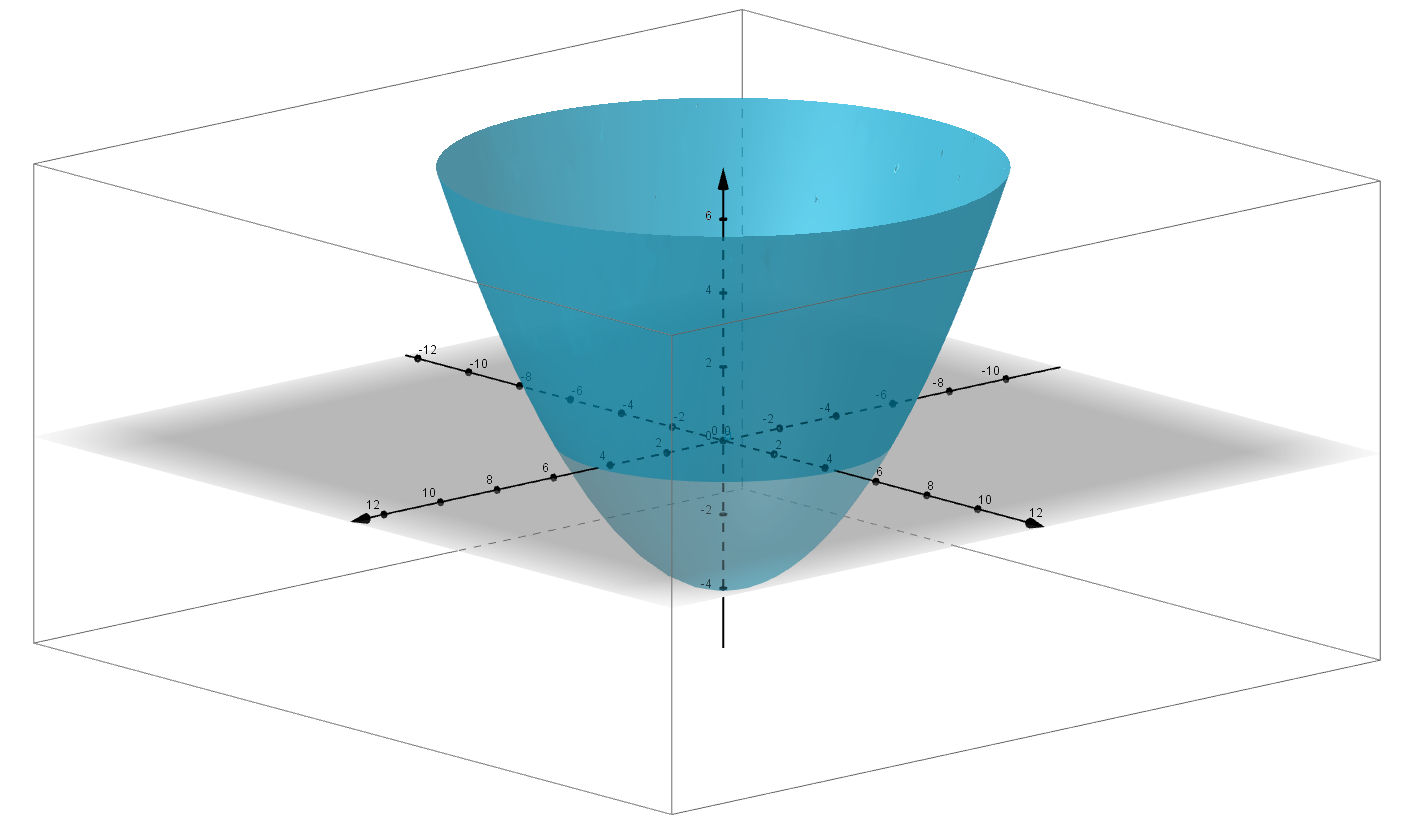
\includegraphics[scale=0.15]{author/grafico_tridim.png}
\captionsetup{font=small, justification=centering}
\caption{Gr\'afico da fun\c c\~ao $f(x,y)$.}
\end{figure}   
\end{trailer}

\subsection{Posicionamento e dimensionamento de figuras}

\noindent O ambiente \verb|figure| tamb\'em permite que possamos reposicionar a figura baseado em alguns comandos. Utilizando \verb|\begin{figure}[onde]|, o argumento “onde” se refere ao local onde deve ser colocada a figura, podendo ser uma combina\c c\~ao das seguintes letras: \\

\begin{itemize}
    \item \textbf{h (here) -} indicará que a figura deve ser inserida exatamente naquele local;
    \item \textbf{t (top) -} indicará que a figura deve ser inserida no topo da próxima página;
    \item \textbf{b (bottom) -}  indicará que a figura deve ser inserida na parte inferior da página;
    \item \textbf{p (page) -} indicará que a figura deve ser inserida em uma p\'agina separada;
    \item \textbf{! -} indicará que devem ser ignorados alguns parâmetros internos e refor\c ca o posicionamento desejado;
    \item \textbf{H -} Caso o \textbf{h} não consiga posicionar uma figura no local desejado nem mesmo com o uso do \textbf{!}, deve-se utilizar o \textbf{H}. Este comando exige o pacote \verb|\usepackage{float}| no preâmbulo. 
\end{itemize}

\noindent Para inclinar uma imagem devemos adicionar o par\^ametro \textit{angle} ao lado do comando \textit{scale} na linha de código \verb|\includegraphics|. O par\^ametro $angle=\theta$ gira a imagem em $\theta$ graus no sentido anti-hor\'ario. Para girar a imagem no sentido hor\'ario, deve-se utilizar um n\'umero negativo. O comando que deve ser utilizado \'e:\\
\vspace{-0.3cm}
\begin{center}
\verb| \includegraphics[scale, angle]{nome da imagem}|.   
\end{center}

\noindent Ao invés de trabalhar apenas alterando a escala das figuras, podemos
redimension\'a-las de outras formas, utilizando como par\^ametros medidas
fixas de largura e/ou altura para a figura. O comando que deve ser utilizado é:
%\vspace{-0.3cm}
\begin{center}
\verb|\includegraphics[width=x cm, height=y cm]{nome da imagem}|,
\end{center}

\noindent onde \textit{widht} indica o comprimento e \textit{height} a altura da figura. Se apenas um dos par\^ametros \textit{width} ou \textit{height} for inserido, o outro ser\'a dimensionado para manter a propor\c c\~ao. 

\subsection{Subfiguras}
Muitas vezes, é necessário incluir várias figuras relacionadas em um mesmo ambiente, como gráficos lado a lado ou imagens que devem ser agrupadas para comparação. A inserção de subfiguras pode ser realizada usando o pacote \texttt{subcaption}, que oferece recursos avançados para criar subfiguras de maneira fácil e personalizável. 

\noindent O pacote \texttt{subcaption} permite criar ambientes de subfiguras dentro de um ambiente \texttt{figure}, permitindo controlar o layout, a legenda e a numeração das subfiguras independentemente. Aqui estão alguns parâmetros comuns usados no ambiente de subfiguras:

\begin{itemize}
    \item \texttt{width}: Define a largura da subfigura. Pode ser especificado em unidades como \verb|cm|.
    \item \texttt{caption}: Define a legenda da subfigura.
    \item \texttt{label}: Define uma etiqueta para referência cruzada.
\end{itemize}

\begin{trailer}{Exemplo}
\begin{verbatim}
\usepackage{graphicx}
\usepackage{subcaption} % Pacote para subfiguras

\begin{document}

\begin{figure}[H]
    \centering

    \begin{subfigure}[b]{0.4\textwidth}
        \centering
        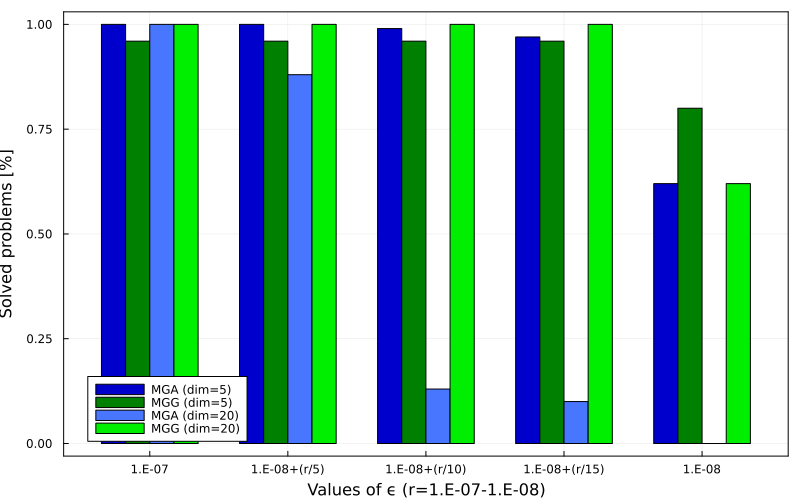
\includegraphics[width=\textwidth]{grafico1.png}
        \caption{Gr\'afico 1.}
    \end{subfigure}
    \hfill
    \begin{subfigure}[b]{0.4\textwidth}
        \centering
        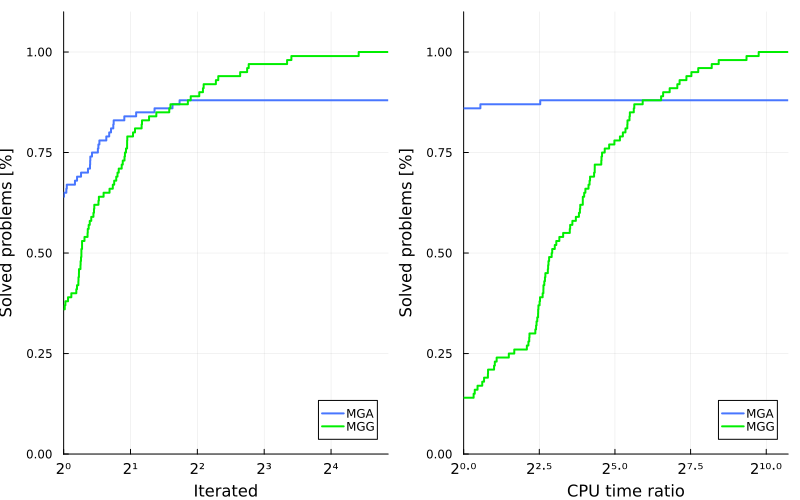
\includegraphics[width=\textwidth]{grafico2.png}
        \caption{Gr\'afico 2.}
    \end{subfigure}
        \begin{subfigure}[b]{0.4\textwidth}
        \centering
        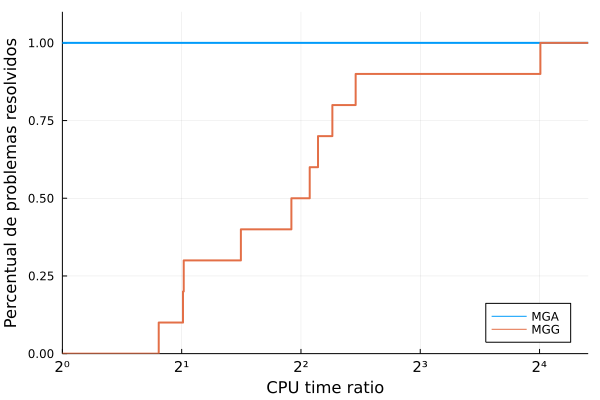
\includegraphics[width=\textwidth]{grafico3.png}
        \caption{Gr\'afico 3.}
    \end{subfigure}

    \caption{An\'alise de gr\'aficos}
    \label{fig:subcaption_example}
\end{figure}

\end{document}
\end{verbatim}   
\end{trailer}

\begin{trailer}{Resultado}
\begin{figure}[H]
    \centering

    \begin{subfigure}[b]{0.4\textwidth}
        \centering
        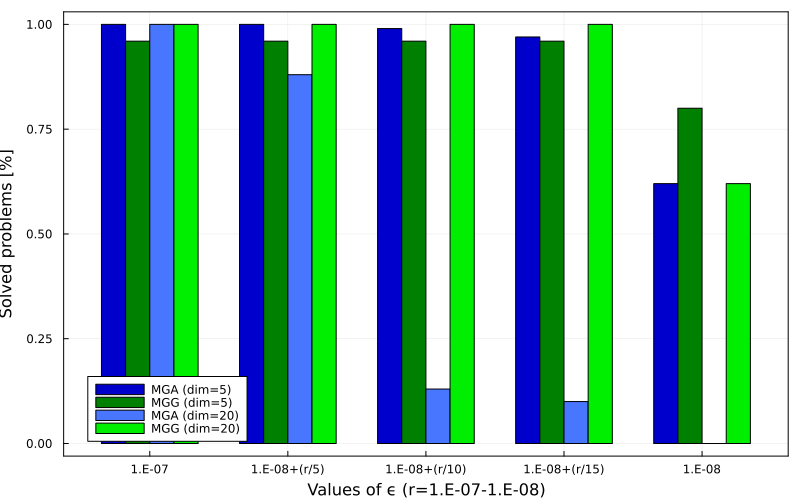
\includegraphics[width=\textwidth]{grafico1.png}
        \caption{Gr\'afico 1.}
    \end{subfigure}
    \hfill
    \begin{subfigure}[b]{0.4\textwidth}
        \centering
        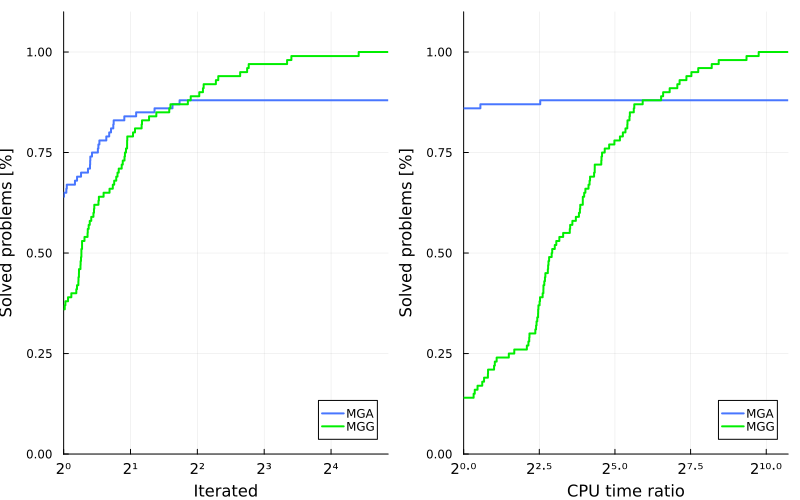
\includegraphics[width=\textwidth]{grafico2.png}
        \caption{Gr\'afico 2.}
    \end{subfigure}
        \begin{subfigure}[b]{0.4\textwidth}
        \centering
        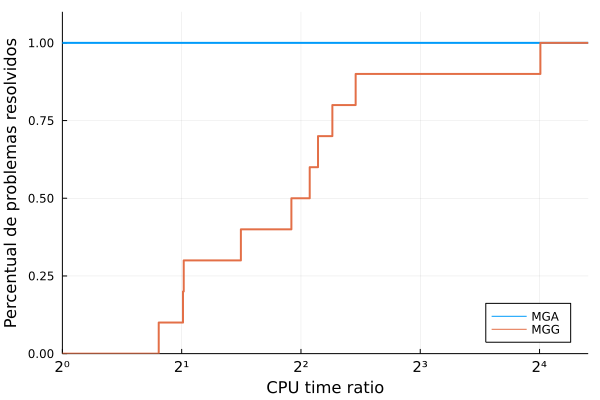
\includegraphics[width=\textwidth]{grafico3.png}
        \caption{Gr\'afico 3.}
    \end{subfigure}

    \caption{An\'alise de gr\'aficos}
    \label{fig:subcaption_example}
\end{figure}    
\end{trailer}

\section{Tabelas}
\label{sec:2}

Tabelas e quadros são elementos essenciais em muitos documentos, pois permitem a organização e apresentação de informações de maneira estruturada. O LaTeX oferece um ambiente poderoso para criar e personalizar tabelas de acordo com suas necessidades.

\subsection{Criação Básica de Tabelas}

Para a cria\c c\~ao de tabelas, deve-se usar o ambiente \texttt{table}. Este ambiente delimita a regi\~ao do c\'odigo onde ser\~ao inseridas as configura\c c\~oes para a tabela. 

\noindent Para inserir a tabela, deve-se usar o ambiente \texttt{tabular} internamente ao ambiente \texttt{table}. Este comando delimita a tabela, para determinar o par\^ametro de n\'umero de colunas. 

\noindent Para o alinhamento do conte\'udo de cada coluna, utilizamos as letras, \textbf{r (right)}, \textbf{l (left)} e \textbf{c (center)} onde \textbf{r} alinha o conteúdo de uma coluna à direita, \textbf{l} à esquerda e
\textbf{c} centraliza. 

\noindent Para determinarmos a quantidade de colunas, basta adicionar um desses par\^ametros para cada coluna e o número de letras de alinhamento ser\'a igual a n\'umero de colunas.

\begin{trailer}{Exemplo}
\begin{verbatim}
\begin{table}[H]
  \centering
  \begin{tabular}{c c}
  célula 1 & célula 2 \\
  célula 3 & célula 4
  \end{tabular}
\end{table}
\end{verbatim}    
\end{trailer}

\begin{trailer}{Resultado}
\vspace{-0.5cm}
\begin{table}
  \centering
  \begin{tabular}{c c}
  célula 1 & célula 2 \\
  célula 3 & célula 4
  \end{tabular}
\end{table}    
\end{trailer}

\subsection{Formatação de Tabelas}
A formatação de tabelas é muito importante para melhorar a legibilidade e a estética. Abaixo estão alguns dos principais comandos de formatação de tabelas.\\

\begin{itemize}
    \item \textbf{Linhas Horizontais:} Use \texttt{\textbackslash hline} para criar linhas horizontais.
    \item \textbf{Colunas Verticais:} Use \texttt{|} entre as letras do argumento do ambiente \texttt{tabular} para criar linhas verticais.
    \item \textbf{Espaçamento:} Use \verb|>{\centering\arraybackslash}p{largura}| para definir espaçamento entre colunas.
\end{itemize}

\begin{trailer}{Exemplo}
\begin{verbatim}
\begin{table}
\centering
\begin{tabular}{|>{\centering\arraybackslash}p{2.5cm}| 
>{\centering\arraybackslash}p{3cm}| 
>{\centering\arraybackslash}p{3.5cm}|}
    \hline
    \textbf{Item} & \textbf{Quantidade} & \textbf{Preço (R\$)} \\
    \hline
    Maçãs & 10 & 2.50 \\
    \hline
    Laranjas & 8 & 3.00 \\
    \hline
    Uvas & 5 & 4.75 \\
    \hline
\end{tabular}
\end{table}
\end{verbatim}   
\end{trailer}

\begin{trailer}{Resultado}
\begin{table}
\centering
\begin{tabular}{|>{\centering\arraybackslash}p{2.5cm}|>{\centering\arraybackslash}p{3cm}|>{\centering\arraybackslash}p{3.5cm}|}
    \hline
    \textbf{Item} & \textbf{Quantidade} & \textbf{Preço (R\$)} \\
    \hline
    Maçãs & 10 & 2.50 \\
    \hline
    Laranjas & 8 & 3.00 \\
    \hline
    Uvas & 5 & 4.75 \\
    \hline
\end{tabular}
\end{table}    
\end{trailer}

\subsection{Mesclagem de Células}

A mesclagem de células pode ser realizada com o pacote \texttt{multirow} para mesclagem vertical e \texttt{multicolumn} para mesclagem horizontal.
\vspace{0.3cm}

\begin{trailer}{Exemplo}
\begin{verbatim}
\begin{table}
\centering
\begin{tabular}{|c|c|c|}
    \hline
    \multicolumn{2}{|c|}{\textbf{Grupo 1}} 
    & \multirow{2}{*}{\textbf{Grupo 2}} \\
    \cline{1-2}
    \textbf{Célula 1} & \textbf{Célula 2} & \\
    \hline
    Dado 1 & Dado 2 & Dado 3 \\
    \hline
    \multirow{2}{*}{\textbf{Células mescladas}} 
    & \multicolumn{2}{c|}{Dado 4} \\
    & \multicolumn{2}{c|}{Dado 5} \\
    \hline
\end{tabular}
\end{table}
\end{verbatim}   
\end{trailer}

\begin{trailer}{Resultado}
 \begin{table}
\centering
\begin{tabular}{|c|c|c|}
    \hline
    \multicolumn{2}{|c|}{\textbf{Grupo 1}} & \multirow{2}{*}{\textbf{Grupo 2}} \\
    \cline{1-2}
    \textbf{Célula 1} & \textbf{Célula 2} & \\
    \hline
    Dado 1 & Dado 2 & Dado 3 \\
    \hline
    \multirow{2}{*}{\textbf{Células mescladas}} & \multicolumn{2}{c|}{Dado 4} \\
    & \multicolumn{2}{c|}{Dado 5} \\
    \hline
\end{tabular}
\end{table}   
\end{trailer}

\subsection{Aparência das tabelas}
V\'arios elementos da tabela podem ser modificados para obter um documento de boa apar\^encia. Pode-se modificar, por exemplo, a espessura, a cor da linha e a cor do plano de fundo das c\'elulas de uma tabela. 

\noindent \'E comum usar duas cores de forma alternada em tabelas para melhorar a legibilidade. Isto pode ser feito em \LaTeX\ com o pacote \texttt{xcolor}, inserindo no pre\^ambulo o comando \verb|{\usepackage[pacote de cores]{xcolor}|. Para inserir as cores, deve-se inserir o comando

\begin{center}
\verb|\rowcolors{\varphi}{cor1! 80! cor2!50 ...}{cor1!70!cor2!40 ...}| 
\end{center}

\noindent antes do ambiente \texttt{tabular}. Esse comando leva tr\^es par\^ametros, cada um dentro de chaves, sendo o primeiro a linha para come\c car a coloriza\c c\~ao, o segundo a cor das linhas \'impares, o terceiro a cor das linhas pares. As cores podem ser misturadas da seguinte forma: o nome da cor seguido de exclama\c c\~ao (exemplo: blue!) e a porcentagem que define sua intensidade em um valor numérico de $0$ a $100$ seguido de exclama\c c\~ao (exemplo: 90!).

% \noindent \textbf{Exemplo:}

% \begin{table}
% \centering
% \rowcolors{1}{}{lightgray}
% \begin{tabular}{|c|c|c|}
%     \hline
%     \textbf{Coluna 1} & \textbf{Coluna 2} & \textbf{Coluna 3} \\
%     \hline
%     Dado 1 & Dado 2 & Dado 3 \\
%     Dado 4 & Dado 5 & Dado 6 \\
%     Dado 7 & Dado 8 & Dado 9 \\
%     \hline
% \end{tabular}
% \caption{Tabela com linhas coloridas alternadas.}
% \end{table}

\noindent Utilizando o comando \verb|\arrayrulecolor|, \'e poss\'ivel colorir as linhas de contorno das tabelas. Este comando deve ser inserido no pre\^ambulo e as cores devem ser inseridas da mesma forma que no pacote \verb|xcolor|.

\noindent Podemos tamb\'em colorir c\'elulas espec\'ificas em uma tabela facilmente atrav\'es do comando \verb|\cellcolor{cores}|. As mesmas observações sobre a sele\c c\~ao de cores mencionadas nos comandos anteriores são v\'alidas para este. Este comando deve ser inserido diretamente na c\'elula que se quer colorir.

\noindent Muitas vezes, a cria\c c\~ao e personaliza\c c\~ao de tabelas no \LaTeX\ podem ser trabalhosas. O site \url{https://www.tablesgenerator.com} \'e uma alternativa para contornar essa dificuldade, pois permite a cria\c c\~ao de tabelas de forma automatizada e gera o c\'odigo em \LaTeX.

\section{Diagramas de Venn}

Os diagramas de Venn s\~ao uma ferramenta visual poderosa para representar rela\c c\~oes entre conjuntos. No \LaTeX, podemos criar esses diagramas usando o pacote \textbf{venndiagram}, que nos permite criar diagramas de Venn de maneira simples e eficaz.

\noindent Primeiramente, o comando \verb|\usepackage{venndiagram}| deve ser inserido no pre\^ambulo.

\noindent Para criar um diagrama de Venn com $2$ conjuntos, pode-se usar o ambiente \verb|venndiagram2sets|. Deve-se usar os comandos \verb|\fillA|, \verb|\fillB| e \verb|\fillAB| para preencher as regi\~oes correspondentes aos conjuntos $A$, $B$ e \`a interse\c c\~ao $AB$, respectivamente.

\begin{trailer}{Exemplo}
\begin{verbatim}
   \begin{venndiagram2sets}    
       \fillA \fillB
   \end{venndiagram2sets}
\end{verbatim}   
\end{trailer}

\begin{trailer}{Resultado}
\begin{center}
   \begin{venndiagram2sets}    
    \fillA \fillB
   \end{venndiagram2sets}
\end{center}   
\end{trailer}

\noindent Para um diagrama com $3$ conjuntos, pode-se utilizar o ambiente \verb|venndiagram3sets| e seguir a mesma estrutura.
%\vspace{0.5cm}

\begin{trailer}{Exemplo}
\begin{verbatim}
   \begin{venndiagram3sets}
       \fillA \fillB \fillC
   \end{venndiagram3sets} 
\end{verbatim}    
\end{trailer}

\begin{trailer}{Resultado}
\begin{center}
   \begin{venndiagram3sets}
    \fillA \fillB \fillC
   \end{venndiagram3sets} 
\end{center}   
\end{trailer}

\noindent O pacote \textbf{venndiagram} oferece várias opções de personalização, incluindo:

\begin{itemize}
    \item \textbf{labelA, labelB, labelC:} Para definir rótulos para os conjuntos.

    \item \textbf{labelOnlyA, labelOnlyB, labelOnlyC:} Para definir rótulos para regiões específicas.

    \item \textbf{labelOnlyAB, labelOnlyAC, labelOnlyBC, labelOnlyABC:} Para rótulos em interseções específicas.
\end{itemize}

\section{Diagramas Comutativos e representa\c c\~ao de Grafos}

\subsection{Diagramas Comutativos}

Um diagrama comutativo \'e uma representa\c c\~ao gr\'afica usada em matem\'atica e outras disciplinas para ilustrar rela\c c\~oes entre objetos e suas transforma\c c\~oes de maneira que o resultado seja independente do caminho escolhido. Em \LaTeX, \'e poss\'ivel criar diagramas comutativos de forma elegante usando pacotes espec\'ificos, como \textbf{tikz-cd}. 

\noindent Para utilizar o pacote \verb|tikz-cd|, você deve inserir no seu pre\^ambulo o comando \verb|\usepackage{tikz-cd}|. O ambiente que ser\'a utilizado \'e o \textbf{tikzcd}. A seguir, mostraremos um exemplo simples.

\begin{trailer}{Exemplo}
\begin{verbatim}
    \begin{tikzcd}
    A \arrow{r}{f} \arrow{d}[swap]{g} & B \\
    C \arrow{ur}[swap]{h}
    \end{tikzcd}
\end{verbatim}   
\end{trailer}

\begin{trailer}{Resultado}
\begin{center}
\begin{tikzcd}
    A \arrow{r}{f} \arrow{d}[swap]{g} & B \\
    C \arrow{ur}[swap]{h}
\end{tikzcd}
\end{center}
\end{trailer}    



\noindent Neste exemplo, temos $3$ objetos: $A$, $B$, $C$ e setas (flechas) que representam as transforma\c c\~oes entre eles. O comando \verb|\arrow| \'e usado para criar flechas e as letras dentro delas representam os nomes das transforma\c c\~oes. A seguir, \'e apresentado um exemplo com $4$ objetos: \\

\begin{trailer}{Exemplo}
\begin{verbatim}
    \begin{tikzcd}
        A \arrow{r}{f} \arrow[swap]{d}{g} & B \arrow{d}{h} \\
        C \arrow{r}{i} & D
    \end{tikzcd}
\end{verbatim}    
\end{trailer}

\begin{trailer}{Resultado}
\begin{center}
\begin{tikzcd}
    A \arrow{r}{f} \arrow[swap]{d}{g} & B \arrow{d}{h} \\
    C \arrow{r}{i} & D
\end{tikzcd}    
\end{center}   
\end{trailer}

\subsection{Grafos}

Os grafos s\~ao uma ferramenta fundamental em matem\'atica e ci\^encia da computa\c c\~ao para representar rela\c c\~oes entre objetos. Em \LaTeX, \'e poss\'ivel criar representações gr\'aficas de grafos usando o pacote \textbf{tikz}, que oferece uma ampla gama de funcionalidades para desenhar grafos personalizados.

\noindent Primeiramente, deve-se inserir no pre\^ambulo o comando \verb|\usepackage{tikz}|.

\noindent Aqui est\~ao alguns conceitos e comandos b\'asicos para a constru\c c\~ao de grafos usando o \textbf{tikz}:

\begin{itemize}
    \item \textbf{Definindo um ambiente de grafo:} Para criar um ambiente para o seu grafo, use o ambiente \textbf{tikzpicture};

    \item \textbf{N\'os (V\'ertices):} Para adicionar n\'os ao seu grafo, use o comando \verb|\node| seguido das coordenadas do n\'o e do nome do n\'o;

    \item \textbf{Arestas:} Para criar arestas entre os n\'os, use o comando \verb|\draw| seguido das coordenadas dos n\'os de origem e destino;
\end{itemize}

\begin{trailer}{Exemplo}
\begin{verbatim}
\begin{tikzpicture}
  \node[draw, circle] (A) at (0,0) {A};
  \node[draw, circle] (B) at (2,1) {B};
  \node[draw, circle] (C) at (2,-1) {C};
  
  \draw[->] (A) -- (B);
  \draw[->] (A) -- (C);
  \draw[->] (B) -- (C);
\end{tikzpicture} 
\end{verbatim}    
\end{trailer}

\begin{trailer}{Resultado}
\begin{center}
\begin{tikzpicture}
  \node[draw, circle] (A) at (0,0) {A};
  \node[draw, circle] (B) at (2,1) {B};
  \node[draw, circle] (C) at (2,-1) {C};
  
  \draw[->] (A) -- (B);
  \draw[->] (A) -- (C);
  \draw[->] (B) -- (C);
\end{tikzpicture}    
\end{center}   
\end{trailer}

\noindent Abaixo segue um exemplo de um grafo com $4$ n\'os:

\begin{trailer}{Exemplo}
\begin{verbatim}
 \begin{tikzpicture}
    \node[draw, circle] (A) at (0, 0) {A};
    \node[draw, circle] (B) at (2, 0) {B};
    \node[draw, circle] (C) at (2, 2) {C};
    \node[draw, circle] (D) at (0, 2) {D};

    \draw[->] (A) -- (B);
    \draw[->] (B) -- (C);
    \draw[->] (C) -- (D);
    \draw[->] (D) -- (A);
\end{tikzpicture}   
\end{verbatim}    
\end{trailer}

\begin{trailer}{Resultado}
\begin{center}
\begin{tikzpicture}
    \node[draw, circle] (A) at (0, 0) {A};
    \node[draw, circle] (B) at (2, 0) {B};
    \node[draw, circle] (C) at (2, 2) {C};
    \node[draw, circle] (D) at (0, 2) {D};

    \draw[->] (A) -- (B);
    \draw[->] (B) -- (C);
    \draw[->] (C) -- (D);
    \draw[->] (D) -- (A);
\end{tikzpicture}     
\end{center}
\end{trailer}

\noindent O \textbf{tikz} permite que você crie grafos mais complexos com diferentes estilos de arestas, cores, formas e tamanhos de n\'os. Voc\^e pode personalizar ainda mais o seu grafo para atender \`as suas necessidades espec\'ificas.

\subsection{Exerc\'icios}

\begin{prob}
    
\end{prob}
\begin{table}[h]
\centering
\caption{Minha Tabela Exemplar}
\label{tab:exemplo}
\begin{tabular}{|c|c|c|c|c|}
\hline
Cabeçalho 1 & Cabeçalho 2 & Cabeçalho 3 & Cabeçalho 4 & Cabeçalho 5 \\ \hline
Dado 1,1 & Dado 1,2 & Dado 1,3 & Dado 1,4 & Dado 1,5 \\ \hline
Dado 2,1 & Dado 2,2 & Dado 2,3 & Dado 2,4 & Dado 2,5 \\ \hline
Dado 3,1 & Dado 3,2 & Dado 3,3 & Dado 3,4 & Dado 3,5 \\ \hline
Dado 4,1 & Dado 4,2 & Dado 4,3 & Dado 4,4 & Dado 4,5 \\ \hline
Dado 5,1 & Dado 5,2 & Dado 5,3 & Dado 5,4 & Dado 5,5 \\ \hline
\end{tabular}
\end{table}

\begin{prob}
    
\end{prob}
\begin{table}[h]
\centering
\caption{Tabela com Mesclagem de Células}
\label{tab:mesclagem}
\begin{tabular}{|c|c|c|c|c|}
\hline
\multicolumn{2}{|c|}{Mesclado 2x1} & Cabeçalho 3 & \multicolumn{2}{c|}{Mesclado 1x2} \\ \hline
Cabeçalho 1 & Cabeçalho 2 & \multirow{2}{*}{Mesclado 2x1} & Cabeçalho 4 & Cabeçalho 5 \\ \cline{1-2} \cline{4-5}
Dado 1,1 & Dado 1,2 & & Dado 1,4 & Dado 1,5 \\ \hline
Dado 2,1 & Dado 2,2 & Dado 2,3 & Dado 2,4 & Dado 2,5 \\ \hline
Dado 3,1 & Dado 3,2 & Dado 3,3 & Dado 3,4 & Dado 3,5 \\ \hline
\end{tabular}
\end{table}

% \section{Conclusão}

%As figuras, tabelas e quadros são elementos cruciais para apresentar informações de maneira organizada e eficaz. O LaTeX oferece uma ampla gama de opções e pacotes para personalizar cada um desses elementos de maneira que atendam às necessidades do seu documento.


%%%%%%%%%%%%%%%%%%%%%%%%% referenc.tex %%%%%%%%%%%%%%%%%%%%%%%%%%%%%%
% sample references
% %
% Use this file as a template for your own input.
%
%%%%%%%%%%%%%%%%%%%%%%%% Springer-Verlag %%%%%%%%%%%%%%%%%%%%%%%%%%
%
% BibTeX users please use
% \bibliographystyle{}
% \bibliography{}
%

\begin{thebibliography}{99.}%
% and use \bibitem to create references.
%
% Use the following syntax and markup for your references if 
% the subject of your book is from the field 
% "Mathematics, Physics, Statistics, Computer Science"
%
% Contribution 
\bibitem{science-contrib} Broy, M.: Software engineering --- from auxiliary to key technologies. In: Broy, M., Dener, E. (eds.) Software Pioneers, pp. 10-13. Springer, Heidelberg (2002)

\bibitem{gratzer2007more}Grätzer, G. (2007). More Math into. New York: Springer.

\bibitem{downes2002short}Downes, M. (2002). Short math guide for LATEX. American Mathematical Society.

\bibitem{stewart2013calculo}Stewart, J. (2011). Calculus. Cengage Learning.

\bibitem{Elon}Lima, E. L. (2004). Análise real (Vol. 1). Rio de Janeiro: Impa.

\bibitem{Tiago}{F. Silva. (2020, October 7). A equação de Schrodinger: Uma mecânica ondulatória. Retrieved September 10, 2023, from \url{https://edisciplinas.usp.br/pluginfile.php/5744597/mod_resource/content/1/Aula%206%20A%20equa%C3%A7%C3%A3o%20de%20Schrodinger.pdf}}

\bibitem{Balino}Baliño. (n.d.). Equação de Navier-Stokes. Retrieved September 14, 2023, from \url{https://edisciplinas.usp.br/pluginfile.php/2967734/mod_resource/content/1/Navier_Stokes.pdf}

\end{thebibliography}


%%%%%%%%%%%%%%%%%%%%% chapter.tex %%%%%%%%%%%%%%%%%%%%%%%%%%%%%%%%%
%
% sample chapter
%
% Use this file as a template for your own input.
%
%%%%%%%%%%%%%%%%%%%%%%%% Springer-Verlag %%%%%%%%%%%%%%%%%%%%%%%%%%
%\motto{Use the template \emph{chapter.tex} to style the various elements of your chapter content.}
\chapter{Bibliografias e Cita\c c\~oes}
\label{intro} % Always give a unique label
% use \chaptermark{}
% to alter or adjust the chapter heading in the running head

Neste capítulo, exploraremos a elaboração de elementos importantes para documentos acadêmicos, incluindo a criação de sumários, índices remissivos e outros recursos relevantes. 

\section{Construção de Sum\'ario}
\label{sec:1}

O \LaTeX{} é projetado para simplificar a criação de documentos estruturados, e isso inclui a geração automática de sumários. Cada vez que \'e criada uma seção, subseção, subsubseção e assim por diante, o \LaTeX{} rastreia essas estruturas para criar uma hierarquia organizada que será usada para gerar o sumário.

\noindent Para criar um sumário, deve-se incluir o comando \verb|\tableofcontents| no local onde \'e desejado que o sumário apareça (normalmente ap\'os o \verb|\begin{document}|, o título e o resumo). Esse comando é responsável por gerar o sumário baseado nas seções e subseções do documento.

\noindent Por padrão, o \LaTeX{} inclui todas as seções, subseções e subsubseções no sumário. Entretanto, é possível personalizar o nível de profundidade exibido no sumário usando o comando \verb|\setcounter{tocdepth}| seguido pelo valor apropriado. Os valores permitidos são de 0 a 3:
\begin{itemize}
    \item 0: Capítulos;
    \item 1: Capítulos e seções;
    \item 2: Capítulos, seções e subseções;
    \item 3: Capítulos, seções, subseções e subsubseções.
\end{itemize}
Por exemplo, para incluir apenas capítulos e seções no sumário, \'e utilizado o seguinte comando:

\begin{trailer}{Constru\c c\~ao de Sum\'ario}
\begin{verbatim} 
\begin{document}
\setcounter{tocdepth}{1}
\tableofcontents  % Gera o sumário
\section{Introdução}
Esta é a introdução do documento.
\subsection{Objetivos}
Nesta subseção, discutimos os objetivos.
\subsubsection{Objetivos específicos}
Nesta subsubseção, discutimos os objetivos específicos. 
\end{document} \end{verbatim}
\end{trailer}

\noindent Para definir o sumário em português, pode-se usar o pacote \verb|babel|, que é um pacote de internacionalização que permite configurar diversos aspectos do documento, incluindo os títulos como "Sumário", "Capítulo", entre outros. Para isso, basta usar \verb|\usepackage[brazilian]{babel}| ou \verb|\usepackage[portuguese]{babel}|.

% O sum\'ario pode ser feito atrav\'es de um \'unico comando que o gera automaticamente. Esse comando \'e o \verb|\tableofcontents|, que deve ser utilizado ap\'os o \verb|\begin{document}|, da seguinte forma: 

% \begin{trailer}{Sum\'ario}
% \begin{verbatim}\begin{document}
% \tableofcontents
% ....\end{verbatim}
% \end{trailer}

\section{Constru\c c\~ao de \'Indice Remissivo}
\label{sec:2}

No \LaTeX{}, o pacote \verb|makeidx| é usado para criar índices remissivos de forma automática. Para ativá-lo, deve-se incluir a seguinte linha no preâmbulo do documento:

\begin{trailer}{Constru\c c\~ao de \'Indice Remissivo}
\begin{verbatim} 
\usepackage{imakeidx}
\makeindex \end{verbatim}
\end{trailer}

\noindent O primeiro comando importa o pacote makeidx, enquanto o segundo comando, \verb|\imakeindex|, instrui o \LaTeX{} a criar o índice remissivo. Para marcar um termo ou palavra para inclusão no índice, basta usar o comando \verb|\index{termo}|, durante o texto que o termo se encontra. Por exemplo:

\begin{trailer}{Inclusão de um termo no \'indice remissivo}
\begin{verbatim} 
O \index{LaTeX} é um sistema de formatação de documentos ...\end{verbatim}
\end{trailer}

\noindent Após marcar os termos relevantes com o comando \verb|\index|, é necessário compilar o documento com uma compilação adicional para que o índice seja gerado.

\noindent Os termos marcados são coletados durante a compilação e organizados em ordem alfabética. Além disso, os números das páginas em que os termos aparecem são registrados. O índice é então inserido no documento no local onde foi colocado o comando \verb|\printindex|. Esta ferramenta é muito importante em textos acadêmicos, pois facilita a busca rápida de informações relevantes no documento.

\section{Constru\c c\~ao de Lista de Figuras e Tabelas}
\label{sec:3}

No \LaTeX{}, é possível gerar automaticamente listas de figuras e tabelas no início do documento, o que torna a navegação do leitor mais fácil e organizada. Para fazer isso, pode-se usar os comandos \verb|\listoffigures| e \verb|\listoftables|. 

\noindent Antes de tudo, deve-se usar o ambiente \verb|figure| para inserir figuras e o ambiente \verb|table| para inserir tabelas, como foi visto no capítulo anterior. Além disso, dentro desses ambientes, é importante utilizar o comando \verb|\caption{}| para adicionar uma legenda descritiva, pois ela aparecerá na lista criada.

\noindent No início do documento, depois do \verb|\tableofcontents| (se houver um sumário), insira os comandos \verb|\listoffigures| e \verb|\listoftables|. Isso fará com que o \LaTeX{} gere automaticamente as listas de figuras e tabelas.

\begin{trailer}{Construção de lista de figuras e de tabelas}
\begin{verbatim} 
\tableofcontents
\listoffigures
\listoftables \end{verbatim}
\end{trailer}

\noindent As legendas usadas com o comando \verb|\caption| serão automaticamente incluídas nas listas de figuras e tabelas. O \LaTeX{} coleta essas legendas e as exibe nas listas correspondentes no início do documento. As listas mostrarão os números das figuras e tabelas, seguidos pelos seus respectivos títulos.

\section{Legendas e Referências cruzadas}
\label{sec:4}

O \LaTeX{} utiliza os ambientes \verb|figure| e \verb|table| para inserir figuras e tabelas, respectivamente. Esses ambientes são "flutuantes", o que significa que o \LaTeX{} decide onde posicioná-los da maneira mais esteticamente agradável, levando em consideração a formatação geral do documento. Dentro dos ambientes \verb|figure| e \verb|table|, o comando \verb|\caption| é usado para adicionar legendas descritivas às figuras e tabelas. Uma legenda deve ser clara e concisa, descrevendo o conteúdo de maneira informativa. 

\noindent O comando \verb|\label| é usado para criar rótulos para figuras e tabelas. Esses rótulos são únicos e permitem criar referências cruzadas para esses elementos em diferentes partes do documento. Veja um exemplo abaixo:

\begin{trailer}{Como rotular uma figura}
\begin{verbatim} 
\begin{figure}[opção]
\includegraphics[opção]{nome.jpg}
\caption{Legenda}
\label{Rótulo}
\end{figure}
\end{verbatim}
\end{trailer}

\noindent Para fazer referência a uma figura ou tabela em outras partes do documento, pode-se usar o comando \verb|\ref|. O \LaTeX{} substituirá automaticamente o número da figura ou tabela correspondente no local da referência. Por exemplo:

\begin{trailer}{Referência cruzada com figura}
\begin{verbatim} 
A Figura \ref{Rótulo} evidencia que...
\end{verbatim}
\end{trailer}

\section{Sistemas de Gerenciamento de Referências}
Os sistemas de gerenciamento de referências, como BibTeX e BibLaTeX, são ferramentas utilizadas para organizar e citar referências bibliográficas em documentos \LaTeX{}. Eles simplificam o processo de gerenciamento, formatação e inclusão de citações. 

\noindent O BibTeX é um sistema tradicional que utiliza arquivos \verb|.bib| para armazenar informações bibliográficas. Cada entrada no arquivo \verb|.bib| descreve um item bibliográfico, como um livro, um artigo, entre outros. Essas entradas têm campos específicos, como autor, título, ano, editora, etc.

\noindent O BibLaTeX é uma evolução do BibTeX, oferecendo capacidades mais avançadas de personalização. Ele é mais flexível na formatação de estilos de citação e é totalmente integrado ao \LaTeX{}. Ele permite estilos de citação altamente personalizados, tornando-o ideal para documentos que seguem diferentes convenções de estilo.

\noindent Para criar um banco de dados bibliográfico no formato \verb|.bib|, pode-se criar um arquivo de texto simples com extensão \verb|.bib|. Cada entrada começa com um tipo (por exemplo, \verb|@book|, \verb|@article|, \verb|@inproceedings|) seguido por campos como \verb|author|, \verb|title|, \verb|year|, etc. Veja exemplos a seguir de entradas \verb|.bib|:

\begin{trailer}{Exemplo de citação para livro}
\begin{verbatim} 
@book{exemploLivro,
    author = {Autor},
    title = {Título do livro},
    year = {ano de publicação},
    publisher = {Editora},
} \end{verbatim}
\end{trailer}

\begin{trailer}{Exemplo de citação para artigo}
\begin{verbatim} 
@article{exemploArtigo,
author = {Autor},
title = {Título do artigo},
year = {ano de publicação},
publisher = {Editora}
} \end{verbatim}
\end{trailer}

\noindent Para inserir a seção de referências utilizando essas ferramentas, basta usar o seguinte comando: 

\begin{trailer}{Criação de Referências}
\begin{verbatim} 
\bibliography{Nome} %Nome do arquivo com extensão .bib
\bibliographystyle{abbrv}
\end{verbatim}
\end{trailer}

\noindent Vale ressaltar que o argumento abbrv utilizado no comando \verb|\bibliographystyle{}| é um estilo de referência, mas é possível utilizar outros estilos. No BibTeX, existem quatro estilos de bibliografia que são comumente utilizados, são eles: \verb|abbrv|, \verb|alpha|, \verb|unsrt| e \verb|plain|. O estilo \verb|abbrv| abrevia os nomes dos autores e títulos dos periódicos. O estilo \verb|alpha| organiza as referências em ordem alfabética. O estilo \verb|unsrt| lista as referências na ordem em que são citadas no texto, sem classificação por ordem alfabética. O estilo \verb|plain| lista as referências na ordem em que são citadas no texto e a entrada da bibliografia pode ser referenciada como [1] ou [ABC20], dependendo das configurações.

\noindent Usando BibTeX ou BibLaTeX, as citações são incorporadas no texto por meio de comandos específicos. No caso do BibTeX, o comando \verb|\cite| é amplamente utilizado. Veja um exemplo abaixo de como inserir a citação no texto:

\begin{trailer}{Citação no texto}
\begin{verbatim} 
Este resultado pode ser visto em \cite{exemploLivro}. \end{verbatim}
\end{trailer}

\noindent Para o BibLaTeX, existem comandos adicionais para maior flexibilidade:

\begin{itemize}
    \item \verb|\parencite{}|: Citação entre parênteses (muito utilizado);
    \item \verb|\textcite{}|: Citação no formato autor-data;
    \item \verb|\footcite{}|: Citação em nota de rodapé.
\end{itemize}

\enlargethispage{24pt}
\include{chapter7}

\backmatter%%%%%%%%%%%%%%%%%%%%%%%%%%%%%%%%%%%%%%%%%%%%%%%%%%%%%%%
% %%%%%%%%%%%%%%%%%%%%%%acronym.tex%%%%%%%%%%%%%%%%%%%%%%%%%%%%%%%%%%%%%%%%%
% sample list of acronyms
%
% Use this file as a template for your own input.
%
%%%%%%%%%%%%%%%%%%%%%%%% Springer %%%%%%%%%%%%%%%%%%%%%%%%%%

\Extrachap{Glossary}


Use the template \emph{glossary.tex} together with the Springer document class SVMono (monograph-type books) or SVMult (edited books) to style your glossary\index{glossary} in the Springer layout.


\runinhead{glossary term} Write here the description of the glossary term. Write here the description of the glossary term. Write here the description of the glossary term.

\runinhead{glossary term} Write here the description of the glossary term. Write here the description of the glossary term. Write here the description of the glossary term.

\runinhead{glossary term} Write here the description of the glossary term. Write here the description of the glossary term. Write here the description of the glossary term.

\runinhead{glossary term} Write here the description of the glossary term. Write here the description of the glossary term. Write here the description of the glossary term.

\runinhead{glossary term} Write here the description of the glossary term. Write here the description of the glossary term. Write here the description of the glossary term.
% 
\Extrachap{Solutions}

\section*{Problems of Chapter~\ref{intro}}

\begin{sol}{prob1}
The solution\index{problems}\index{solutions} is revealed here.
\end{sol}


\begin{sol}{prob2}
\textbf{Problem Heading}\\
(a) The solution of first part is revealed here.\\
(b) The solution of second part is revealed here.
\end{sol}


% \printindex
%%%%%%%%%%%%%%%%%%%%%%%% referenc.tex %%%%%%%%%%%%%%%%%%%%%%%%%%%%%%
% sample references
% %
% Use this file as a template for your own input.
%
%%%%%%%%%%%%%%%%%%%%%%%% Springer-Verlag %%%%%%%%%%%%%%%%%%%%%%%%%%
%
% BibTeX users please use
% \bibliographystyle{}
% \bibliography{}
%

\begin{thebibliography}{99.}%
% and use \bibitem to create references.
%
% Use the following syntax and markup for your references if 
% the subject of your book is from the field 
% "Mathematics, Physics, Statistics, Computer Science"
%
% Contribution 
\bibitem{science-contrib} Broy, M.: Software engineering --- from auxiliary to key technologies. In: Broy, M., Dener, E. (eds.) Software Pioneers, pp. 10-13. Springer, Heidelberg (2002)

\bibitem{gratzer2007more}Grätzer, G. (2007). More Math into. New York: Springer.

\bibitem{downes2002short}Downes, M. (2002). Short math guide for LATEX. American Mathematical Society.

\bibitem{stewart2013calculo}Stewart, J. (2011). Calculus. Cengage Learning.

\bibitem{Elon}Lima, E. L. (2004). Análise real (Vol. 1). Rio de Janeiro: Impa.

\bibitem{Tiago}{F. Silva. (2020, October 7). A equação de Schrodinger: Uma mecânica ondulatória. Retrieved September 10, 2023, from \url{https://edisciplinas.usp.br/pluginfile.php/5744597/mod_resource/content/1/Aula%206%20A%20equa%C3%A7%C3%A3o%20de%20Schrodinger.pdf}}

\bibitem{Balino}Baliño. (n.d.). Equação de Navier-Stokes. Retrieved September 14, 2023, from \url{https://edisciplinas.usp.br/pluginfile.php/2967734/mod_resource/content/1/Navier_Stokes.pdf}

\end{thebibliography}

%%%%%%%%%%%%%%%%%%%%%%%%%%%%%%%%%%%%%%%%%%%%%%%%%%%%%%%%%%%%%%%%%%%%%%

\end{document}





